\chapter{Measurement of W plus \bbbar Pair Production}
This document describes a study of W boson production
in association with two b quarks, where W bosons are observed via their decays to muons, and
b quarks are identified as two separated jets.
This production channel provides an important testing ground for 
%perturbative electroweak and 
%QCD calculations as implemented in the 
standard model (SM) predictions. 
Previous
measurements of vector boson production with associated b jets
~\cite{Aaltonen:2009qi,D0:2012qt,Aad:2011kp} have shown varying levels of agreement with theoretical 
calculations.
The precise experimental measurement of the $\Wbb$ cross section will therefore provide important
input to refine theoretical calculations in perturbative QCD, as well as validate associated Monte Carlo techniques.
Understanding the  production of $\Wbb$ events is also crucial as they constitute a major background in the
study of processes with two 
separated and well identified b jets in the final state, one of which is
the search for the standard model Higgs boson (H) decaying to $\bbbar$
when produced in association with a weak vector boson.

The analysis uses a sample of proton-proton collisions 
at a center-of-mass energy of $\sqrt{s}$=7 TeV collected in 2011 with the CMS experiment at the LHC, 
corresponding to an 
integrated luminosity of $5.0\fbinv$.
While the CMS detector is described in detail elsewhere~\cite{CMSExperiment}, the
key components for this analysis are summarized here.
The CMS experiment uses a right-handed coordinate system, with the
origin at the nominal interaction point, the x-axis
pointing to the center of the LHC ring, the y-axis pointing
up (perpendicular to the plane of the LHC ring), and the z-axis
along the counterclockwise-beam direction. The polar angle
$\theta$ is measured from the positive z-axis and the
azimuthal angle $\phi$ is measured in the x-y plane.
The absolute value of the transverse
momentum ($\pt$) is calculated as 
$\pt = \sqrt{p_{\rm{x}}^2 + p_{\rm{y}}^2}$.
%%%
A superconducting solenoid occupies the
central region of the CMS detector, providing an axial magnetic
field of 3.8~T parallel to the beam direction.
The silicon pixel and strip
tracker, the crystal electromagnetic calorimeter, and the brass/scintillator hadron
calorimeter are located within the solenoid. A quartz-fiber
Cherenkov calorimeter extends the coverage to $|\eta| <$ 5.0, where pseudorapidity
is defined as $\eta=-{\rm ln}[\tan{(\theta/2)}]$.
Muons are measured in gas ionization detectors embedded 
in the steel flux return yoke outside the solenoid.
The first level of the CMS trigger system, composed of custom
hardware processors, is designed to select the most interesting events
in less than 3 $\mu$s using information from the calorimeters and muon
detectors. 
The high-level-trigger processor farm decreases the event rate from 100 kHz
delivered by the first level trigger to a few hundred hertz, before data storage.

A number of Monte Carlo (MC) event generators are used to simulate the signal and
backgrounds. 
The  events with W or Z boson production, or with $\ttbar$ production, are generated at leading order (LO) 
with \MADGRAPH 5.1~\cite{Madgraph5}, which is interfaced with \PYTHIA 6.4~\cite{Sjostrand:2006za} (also LO)
for hadronization.
Single top samples are generated at next-to-leading order (NLO) with 
\POWHEG2.0~\cite{Alioli:2008gx,Nason:2004rx,Frixione:2007vw}.
Diboson ($\WW$, $\WZ$, $\ZZ$) and multijet samples are
generated with 
\PYTHIA 6.4~\cite{Sjostrand:2006za}. 
For LO generators, the default set of parton distribution functions
(PDF) used to produce these samples is CTEQ6L~\cite{CTEQ66}, while
MSTWNNLO~\cite{Martin:2009iq} is used for NLO generators.
For all processes, the detector response is simulated using a detailed
description of the CMS detector, based on the \GEANTfour~
package~\cite{GEANT}, and event reconstruction is performed with
the same algorithms as used for data.
The simulated samples include additional interactions per bunch crossing (pileup),
the distribution for which comes from data.
Parton showering is simulated with PYTHIA using the Z2 tune~\cite{Field:2010bc}.

A complete reconstruction of the individual particles emerging from each collision event is obtained 
via a particle-flow (PF) technique~\cite{CMS-PAS-PFT-09-001, CMS-PAS-PFT-10-002}. This 
approach uses the information from all CMS sub-detectors to identify and 
reconstruct individual particles in the collision event, classifying 
them into mutually exclusive categories: charged hadrons, neutral hadrons, photons, electrons, and muons.

Muons are reconstructed~\cite{CMS-PAS-MUO-10-002}
by combining the information of the tracker and the muon spectrometer.
The muon candidates are required to be compatible with the primary vertex of the
event, which is chosen as the vertex with highest $\sum \pt^2$ of its associated tracks.
The muon relative isolation is defined as
\begin{equation*}
I^{\rm{rel}} = \left( \sum_{i}
p_{\text{T, charged}}^i+ \sum_{j}  E_{\text{T, photon}}^j  +\sum_{k}  E_{\text{T, neutral}}^k \right) /\pt^{\mu},
\end{equation*}
with the sums running over all the charged and neutral PF candidates,
excluding the muon candidate itself, 
within a cone around the muon direction
defined by  $\Delta R  < \Delta R_{\rm max} = 0.4$,
where
$\Delta R = \sqrt { (\Delta \eta)^2 + (\Delta \phi)^2 }$, and
\ET stands for the
transverse energy.
%A muon isolation variable, $I^{\rm{rel}}$, is calculated as a 
%sum of the transverse energies  momenta of reconstructed PF particles in a 
%around the direction of the muon, normalized to the muon momentum,
%and excluding the contribution from the lepton candidate itself. 
%The muon is required to be isolated
%from any other detector activity according to the criterion $I^{rel}<0.12$. 

These identified, isolated muons are then combined with the missing transverse 
energy $\vecEtm$ of the event to form a leptonic W candidate. 
The missing transverse energy $\vecEtm$ is defined as
the negative vector sum of the
transverse momenta of all reconstructed particles in the event, with $\MET = |\vecEtm|$,
and is corrected using the procedure 
described in Ref.~\cite{WZCMS:2010}.
The reconstructed transverse mass of the system is built from the transverse momentum of the isolated muon 
and the missing transverse energy of the event, 
\begin{equation*} 
M_\mathrm{T} = \sqrt{2 \pt^{\ell} \MET (1-\cos \Delta \phi)}\ ,
\nonumber
\end{equation*}
where
$\Delta \phi$
is the difference in azimuth between $\vecEtm$ and $\vecPtmu$. In $\Wln$ decays the $M_T$ distribution presents a Jacobian peak 
with an edge at the W mass. Therefore it is a natural topological discriminator against non-W final states which yield a lepton candidate and
missing transverse energy, such as QCD multijet processes, 
in which the events concentrate at low values of the $M_T$ variable. 

Jets are reconstructed from the PF candidates.
The anti-$\mathrm{k_T}$
clustering algorithm~\cite{Cacciari:2008gp} with distance parameter of 0.5
is used, as implemented in the \textsc{fastjet}
package~\cite{fastjet1,fastjet2}. 
%The jet energy is corrected
%for pileup in a manner similar to the correction of the energy inside a lepton
%isolation cone. 
Jets are required to pass identification
criteria that eliminate jets originating or being seeded by
noisy channels in the calorimeter~\cite{Chatrchyan:2009hy}.
In addition to this, jets originating from pileup interactions are
rejected by requiring compatibility of the jets 
with the primary interaction vertex. 
Jet energy corrections are also applied as a function of the jet
$\pt$ and $\eta$~\cite{cmsJEC}.

Secondary vertices (SV) are reconstructed inside each jet.
% using the trimmed kalman vertex 
%finder~\cite{XXX}.
This study makes use of the combined secondary vertex (CSV) b-tagging algorithm~\cite{refCSV};
this algorithm makes use of the
long lifetime and high mass of b hadrons
to provide optimized 
b-quark jet discrimination,
by combining information 
about impact parameter significance, secondary vertex, and 
jet kinematics in a likelihood ratio technique. B-tagged jets are selected by imposing a 
minimum threshold on the CSV discriminator value.
The analysis is based on a CSV
discriminator threshold
which provides an efficiency of approximately 50$\%$  for identifying
jets containing b-flavored hadrons while reducing the misidentification probability for light-quark jets to 0.1$\%$~\cite{BTAGNOTE}
%%%% Note that TOP-12-024 quotes 45% - 0.1% 


\begin{figure}
\centering
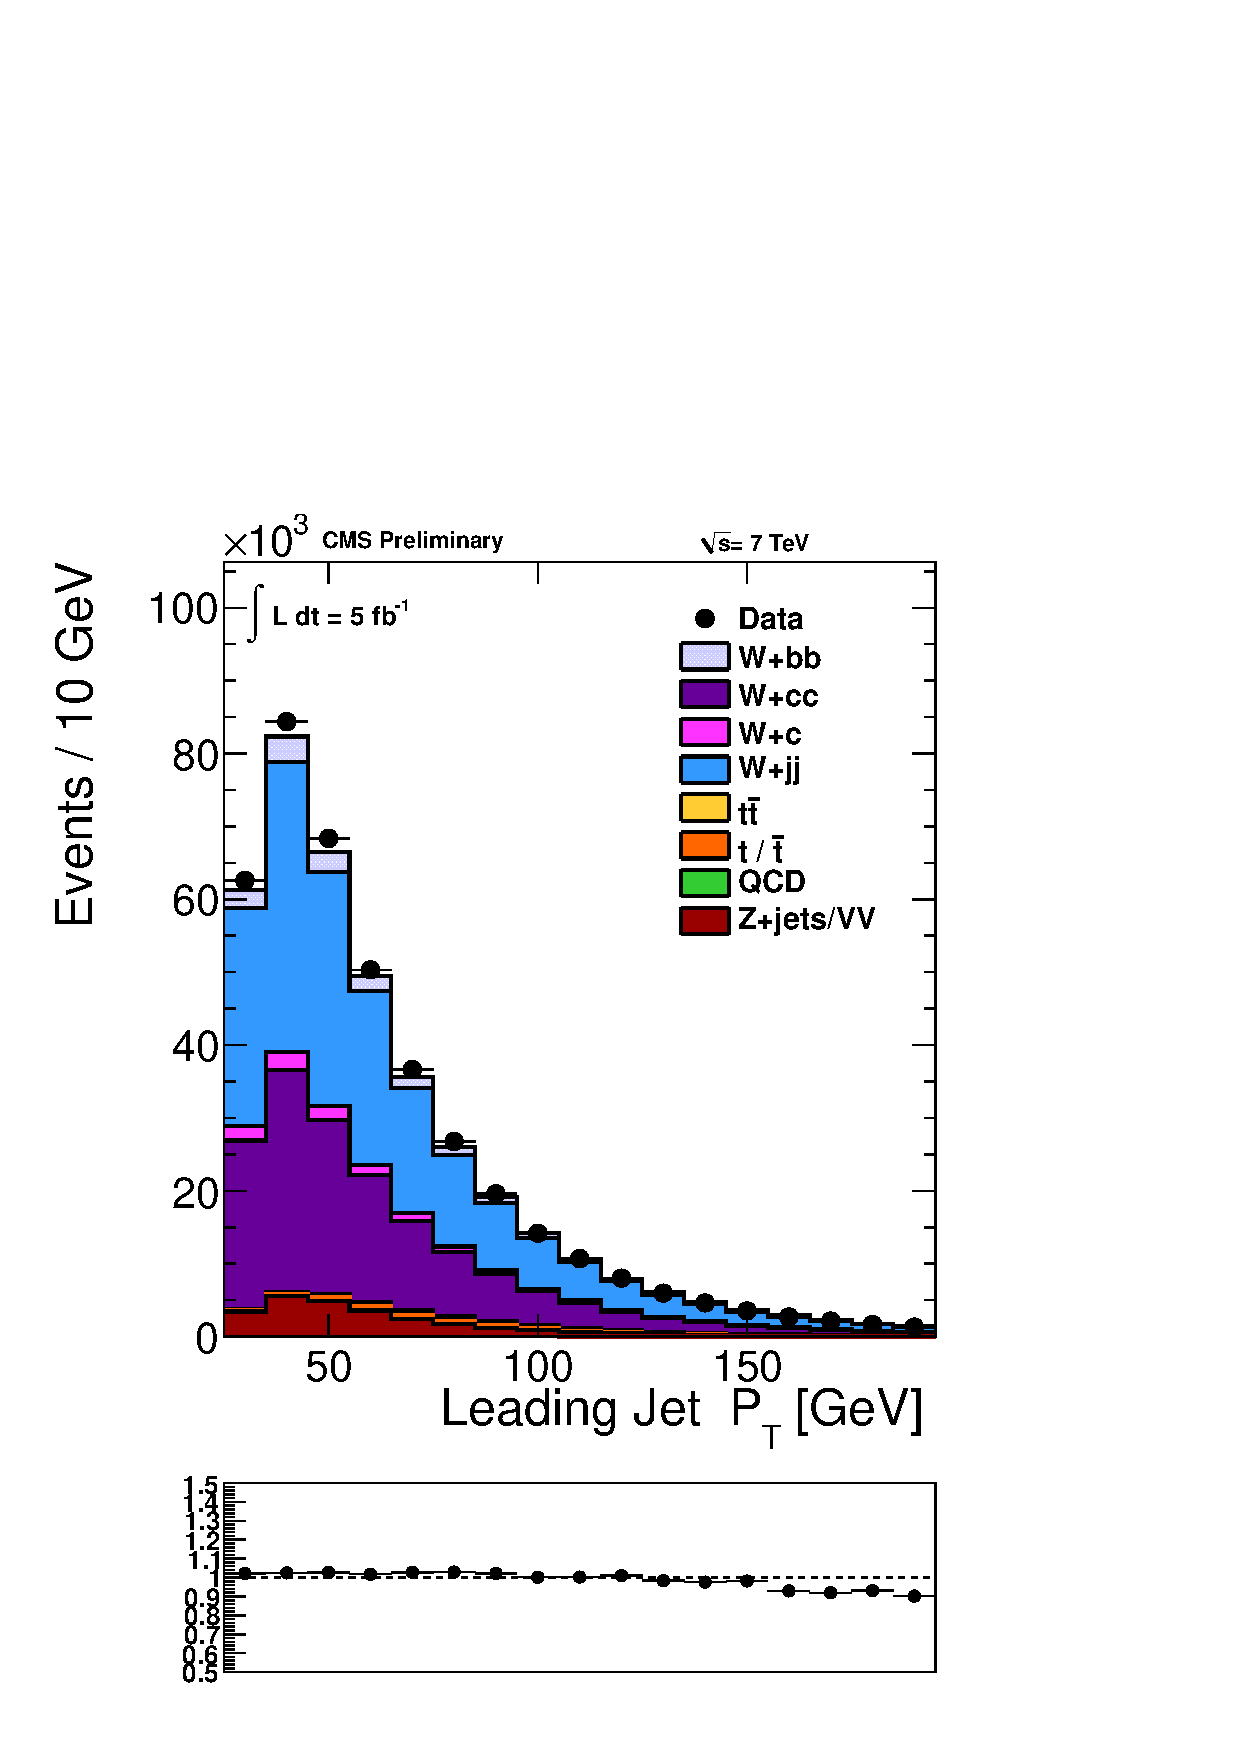
\includegraphics[width=0.45\textwidth, trim = 0 4cm 0 0, clip=true ]{Wbb/fig1.pdf}
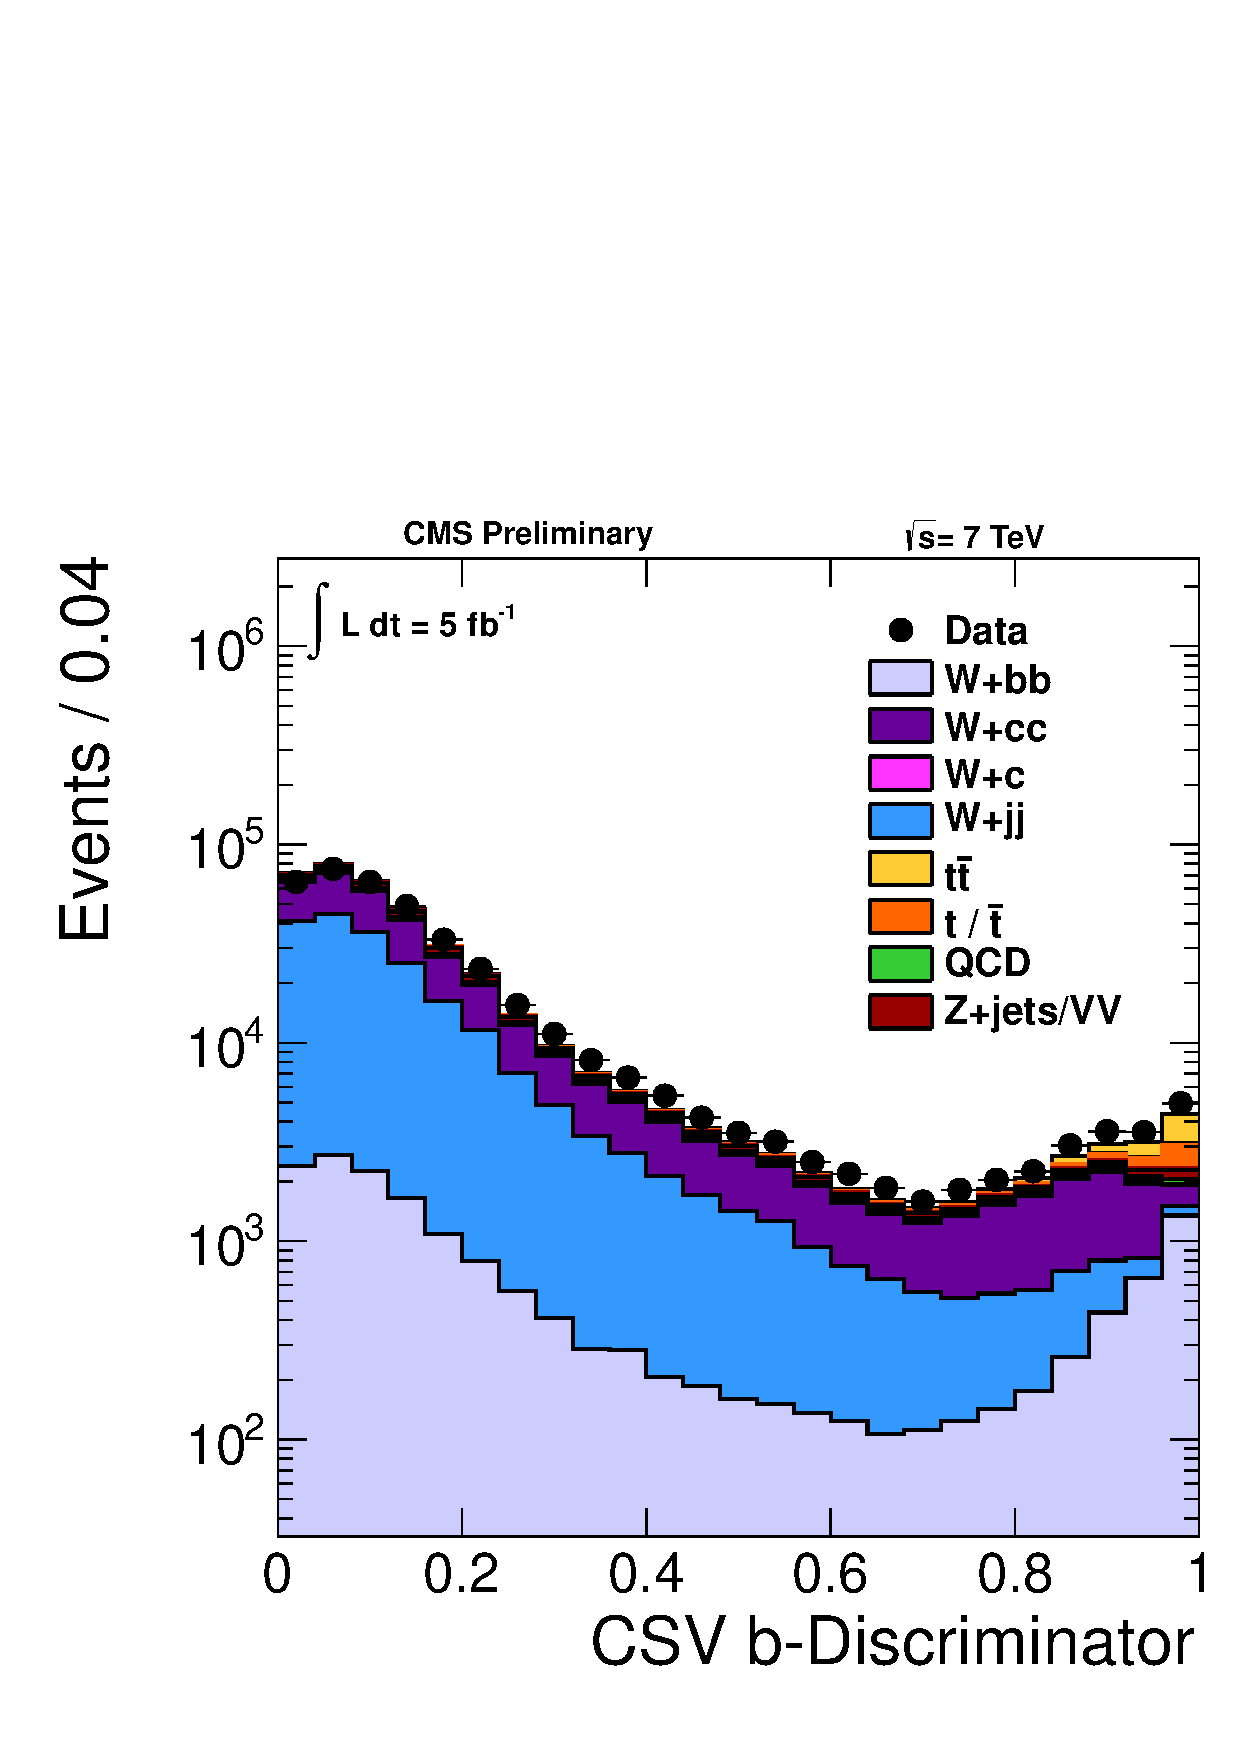
\includegraphics[width=0.45\textwidth]{Wbb/fig1_jetcsv.pdf}

\caption{(left) The highest-$p_{T}$ jet ($\rm{J_{1}}$) before applying b-tagging.
(right) The CSV b-discriminator 
for $\rm{J_{1}}$.}
\label{fig:figA}
\end{figure}


%The b-tagging working point
%chosen for the analysis is the tight one, in which the efficiency of the selection is approximately 60$\%$, 
%while a suppression
%factor for jets from light quarks is approximately 100~\cite{cmsBTAGPAPER}.

The $\Wbb$ selected events are required to have  
an isolated muon with $I^{\rm{rel}}<0.12$, $\pt>25\GeV$, $|\eta|<2.1$,
exactly two jets with $\pt>25\GeV$ and $|\eta|<2.4$, where 
both selected jets must contain a secondary vertex 
and pass the b-tagging CSV requirement.
To reduce the contribution from Z-boson production, the 
event is rejected if there is a second muon, without any requirements 
on the isolation and $\pt$, 
which builds with the isolated muon a dimuon system with 
invariant mass $m_{\mu\mu} > 60\GeV$. 
The $\ttbar$ background is reduced by requiring
that there are no additional isolated electrons or muons with  $p_{T}>20\GeV$ in the event and no
jets with $\pt>25\GeV$ and $2.4<|\eta|<4.5$. To reduce the contribution
from QCD multijet events $\MT > 45\GeV$ is also required.

After all the selection requirements the significant background 
contributions are:
$\ttbar$, single top, W+jets (u,d,c,s,g), Z+jets (u,d,c,s,b,g) and QCD multijet. 
Contributions of all these backgrounds 
are computed in 
a simultaneous fit, which provides a final estimate for the signal and background yields.

With the exception of QCD, the shapes of the background distributions are taken from simulation. 
A shape for the QCD contribution is obtained directly from  data  from 
a multijet-enriched control region
defined by all the selection requirements, but
requiring the muon to be non-isolated ($I^{\rm{rel}}>0.2$). The QCD uncertainty in the 
final fit is taken to be $\pm$50\%. This uncertainty is large enough to provide coverage for 
normalization and shape mismodelings of the small QCD contribution in the final sample.
% comes directly from the uncertainty on the
%fit in the QCD background-enriched control region.

The initial yields are taken either from data, in estimates based on the 
control regions, or from simulation, normalized to the NNLO predictions.
The shapes and normalizations of the background distributions
are validated in data with a set of control regions.

The W+$\rm{jets}$ (u,d,c,s,g) process, where the jets are not initiated by b quarks,
is the dominant background before applying the selection requirements on the secondary vertex and
b-tagging. Figure~\ref{fig:figA} (left) shows the $\pt$ of the leading jet at 
this preselected stage. The CSV algorithm working point which provides maximum reduction of 
W+$\rm{jets}$ (u,d,c,s,g) is used. 
The CSV b-tagging discriminant for the leading jet is shown in Figure~\ref{fig:figA} (right). The presence of light and charm jets
in the sample is very small at the higher values of the discriminant.
Furthermore, to increase the purity of the sample %maximally reduce the contribution from the $\Wcc$ process 
a secondary vertex is required to be reconstructed in each of the selected jets.
Figure~\ref{fig:figAbis} shows the mass of the secondary vertex of the leading jet ($\rm{J_{1}}$, right) and the sub-leading jet ($\rm{J_{2}}$, left), for the final selection
in the signal region.
These selection requirements have been validated in the $\ttbar$ and Z+jets control regions
described below. 
%in the $\cPZ$+bb and $\ttbar$ control regions. 
%The number of secondary vertices before b-tagging for the signal region region is plotted in Figure~\ref{fig:fig}.

\begin{figure}
\centering
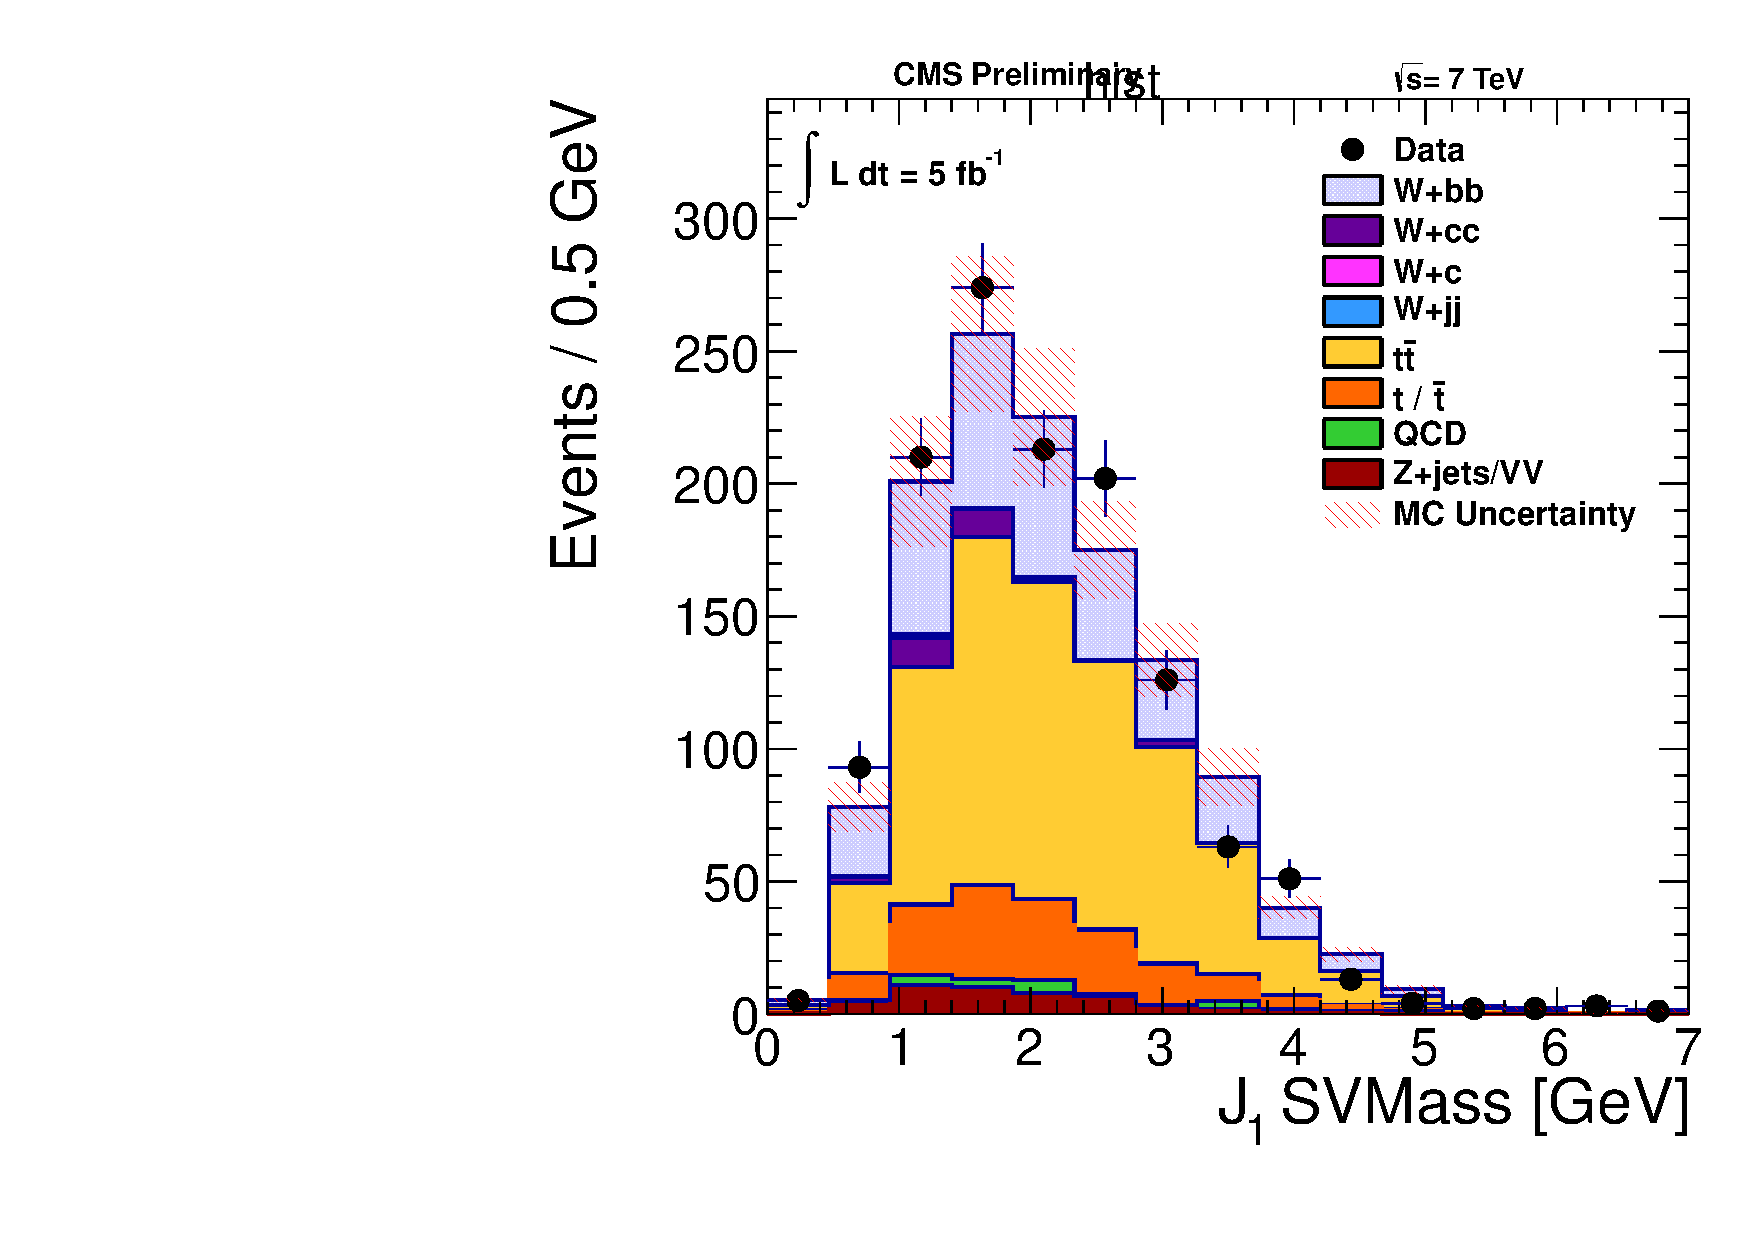
\includegraphics[width=0.47\textwidth]{Wbb/fig1a_J1Mass.pdf}
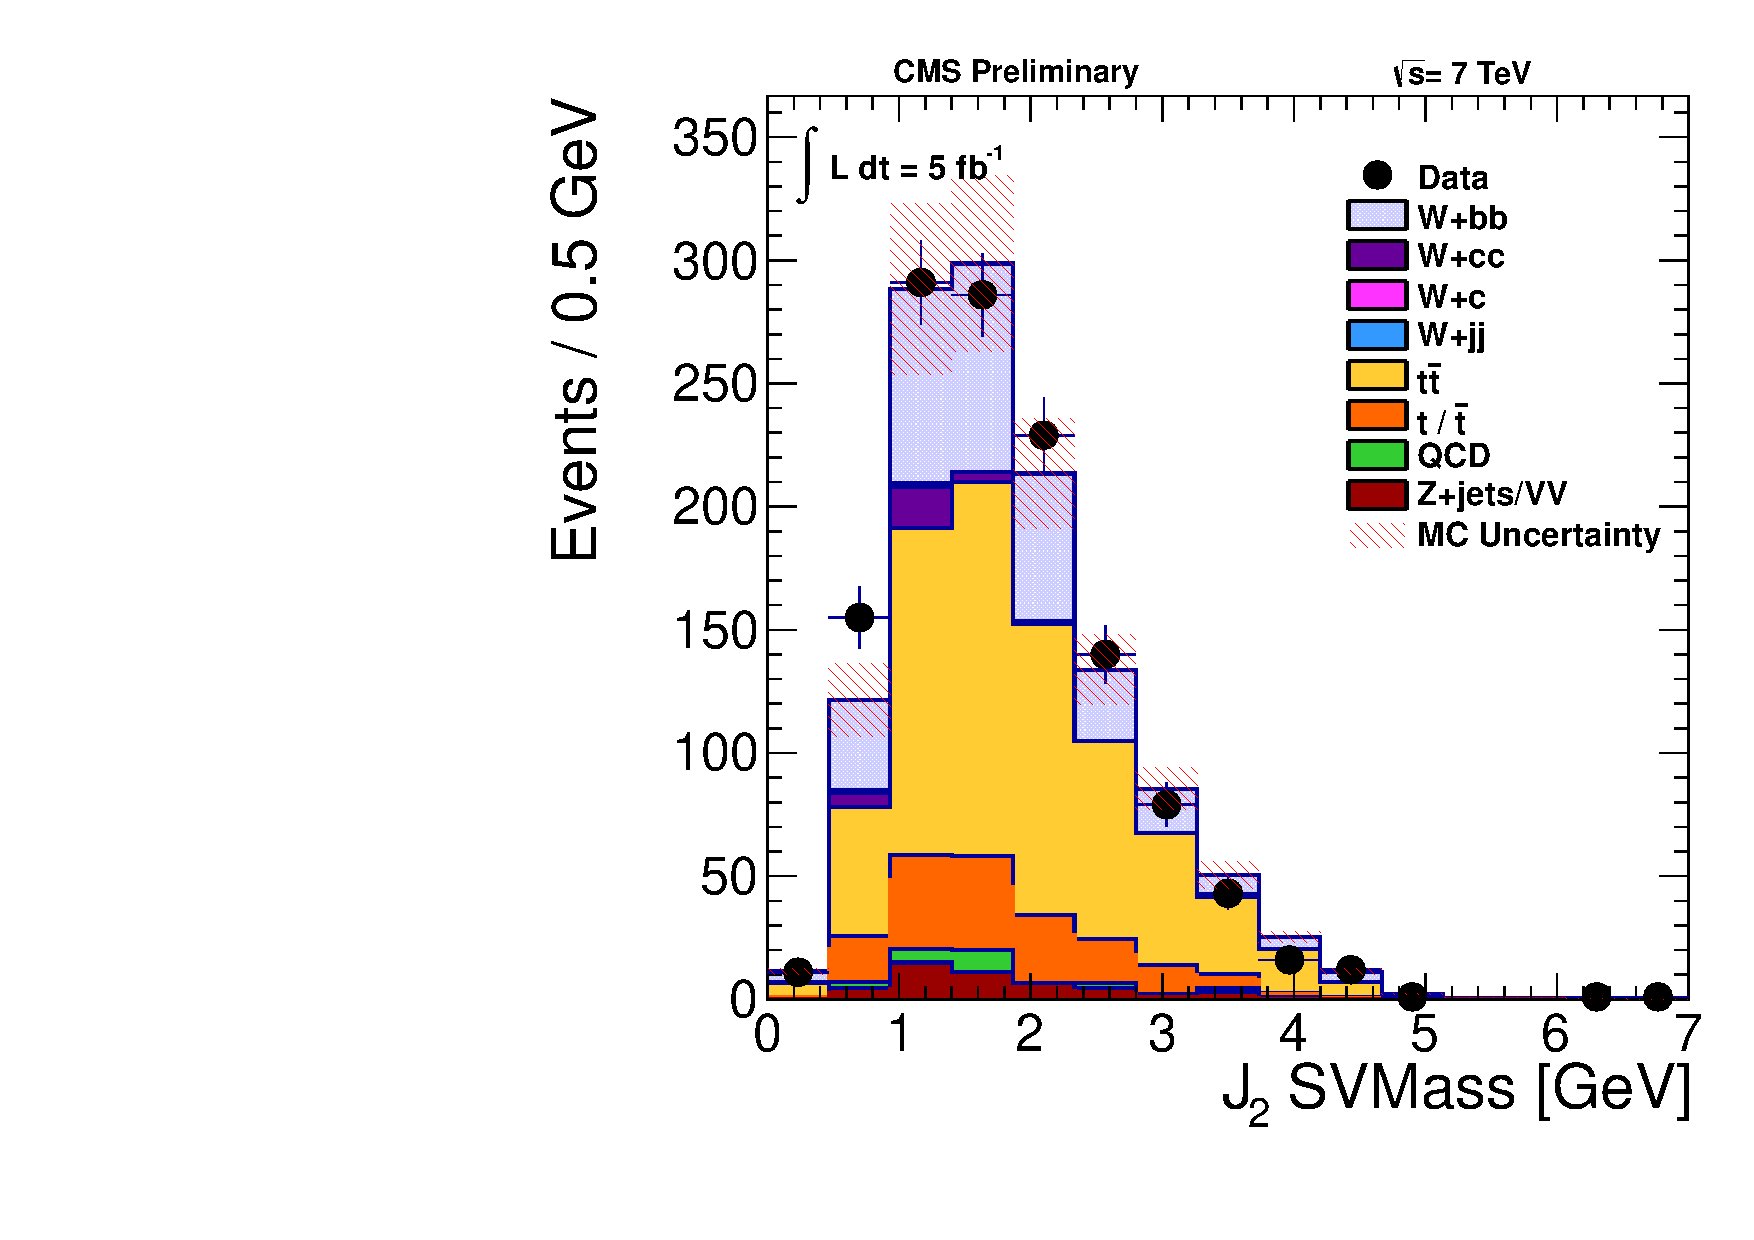
\includegraphics[width=0.47\textwidth]{Wbb/fig1a_J2Mass.pdf}
\caption{Mass of the secondary vertex for the highest-$p_{T}$ jet ($\rm{J_{1}}$, right) and for the second jet ($\rm{J_{2}}$, left) in the signal region.}
\label{fig:figAbis}
\end{figure}

The events selected for the $\ttbar$ control region pass the selection requirements, with
no restrictions on the number of leptons in the event. 
In addition to the two highest-$\pt$ b-tag jets, the events are required to have at least two extra light jets.
This higher jet multiplicity requirement selects a sample that is dominated by $\ttbar$ events.
Figure~\ref{fig:figB} (right) shows the invariant mass of the 
two highest-$\pt$ additional jets (3rd and 4th highest-$\pt$ in the event, $m_{\rm{J_{3}J_{4}}}$). 
In $\ttbar$ events this distribution reconstructs the mass of the hadronically decaying W boson. 
It is used in the final fit to extract the $\ttbar$ background normalization.
% CHECK: Add info on JES? JER?
The simulation describes the observed distributions well both in 
shape and normalization.
%\begin{figure}
%\centering
%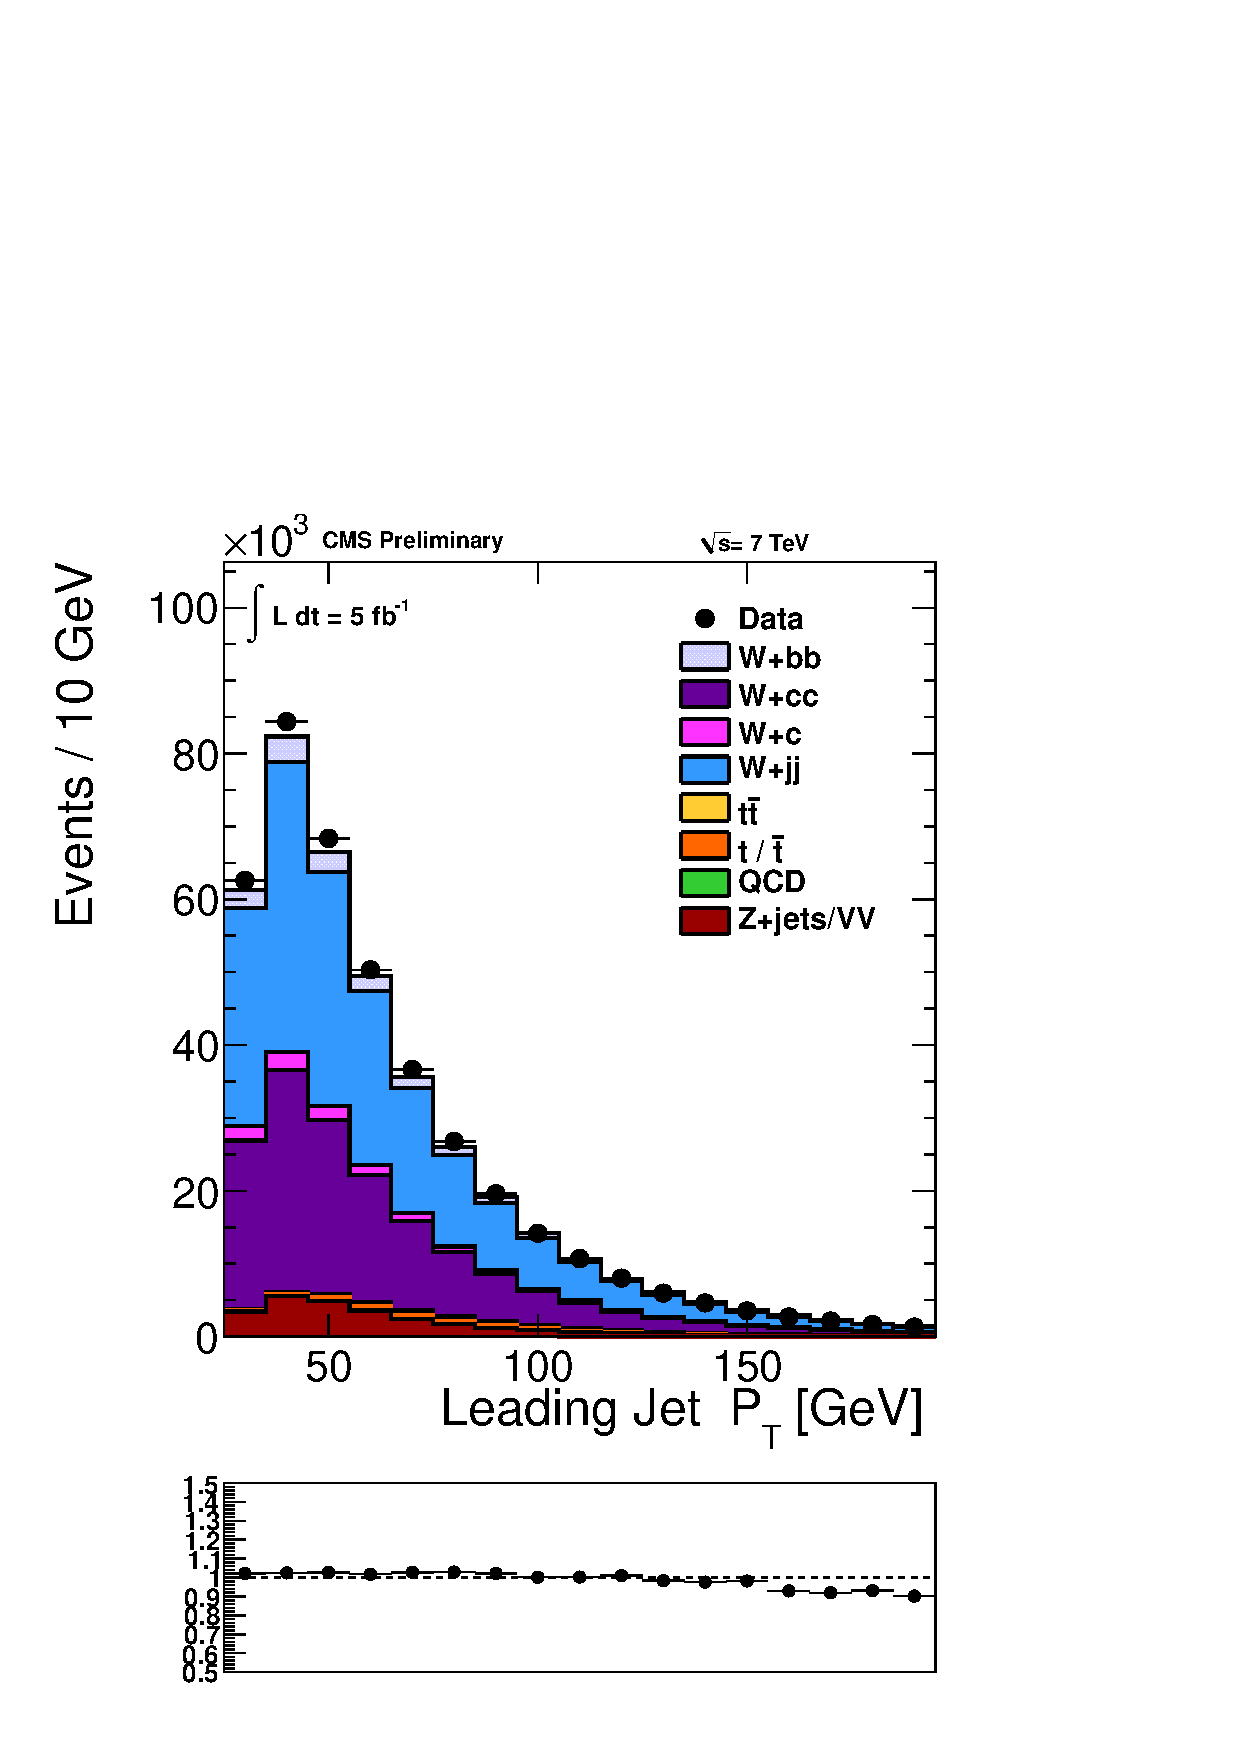
\includegraphics[width=0.45\textwidth,trim = 0 4cm 0 0, clip=true ]{Wbb/fig1.pdf}
%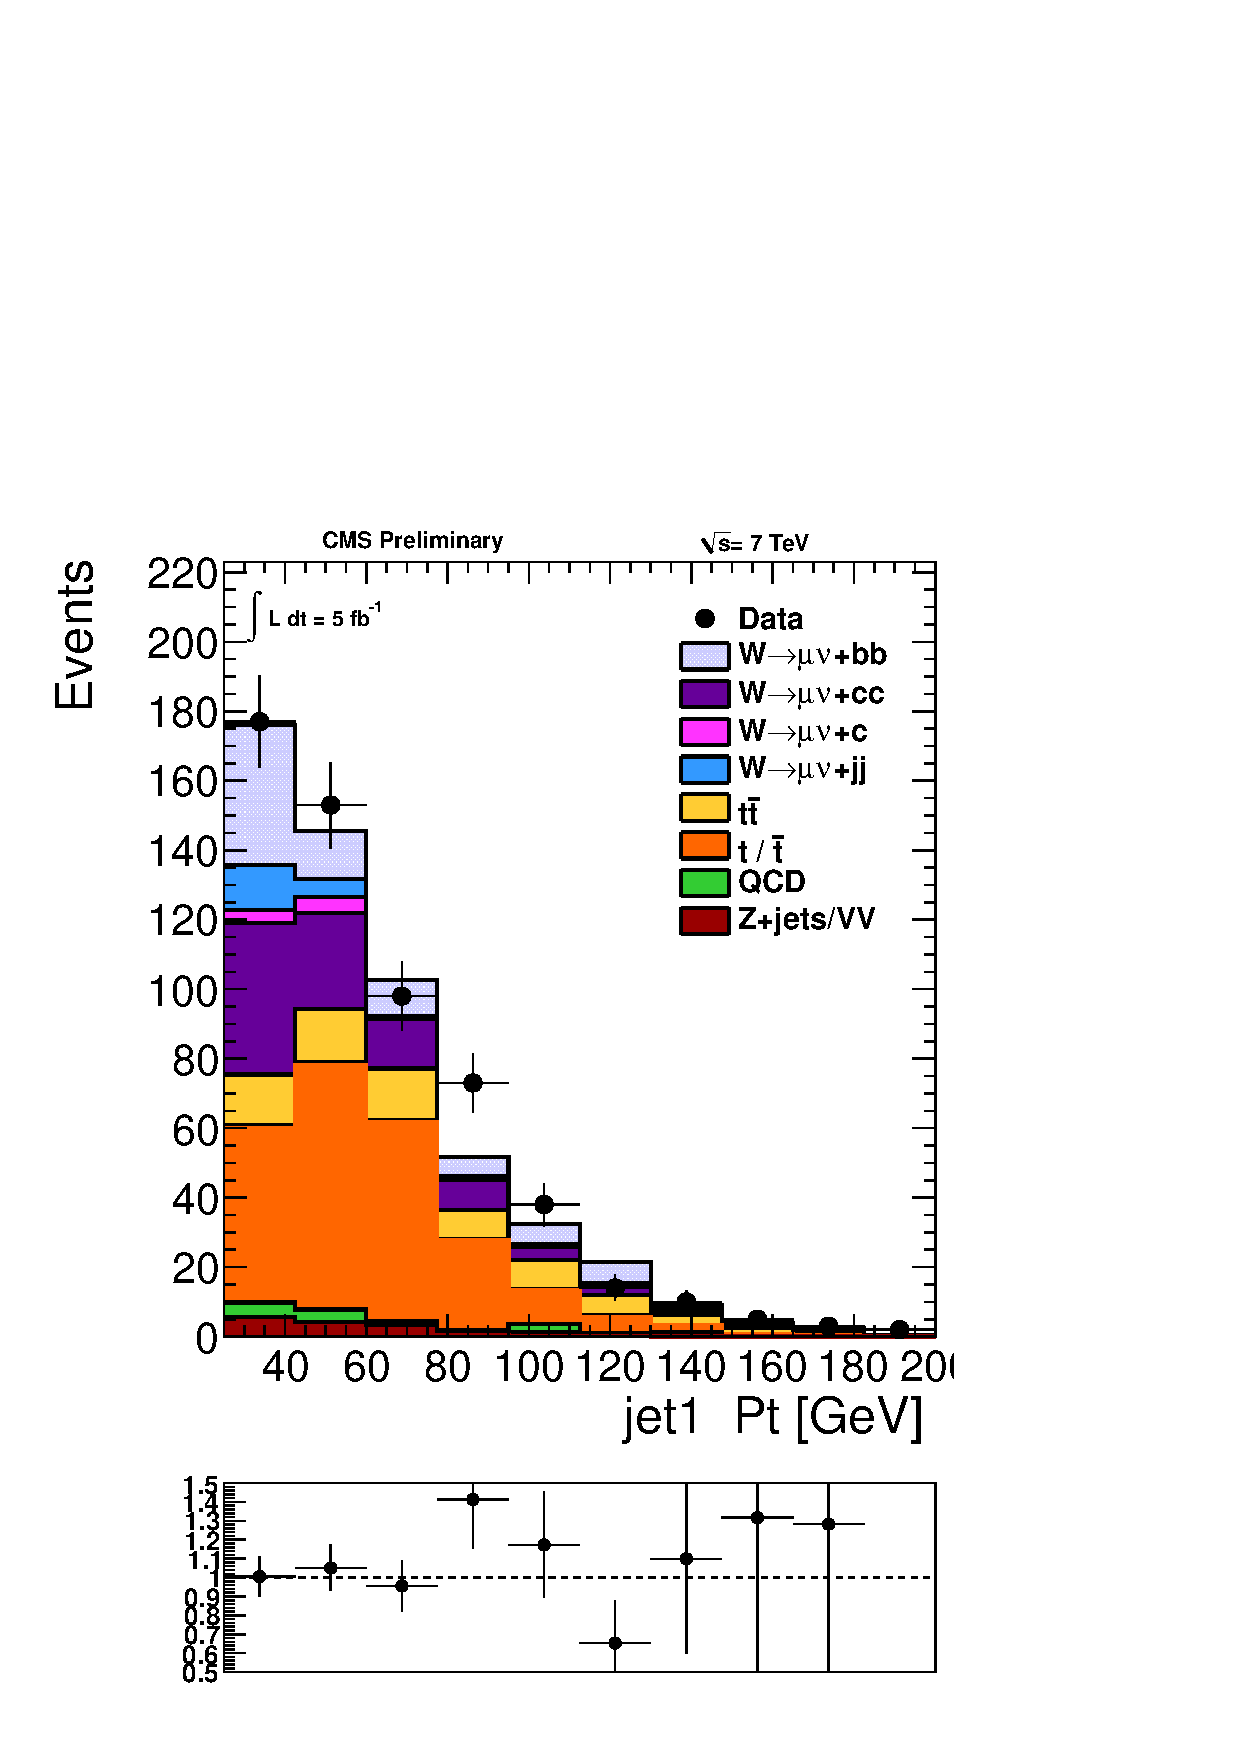
\includegraphics[width=0.45\textwidth,trim = 0 4cm 0 0, clip=true ]{Wbb/fig2.pdf}
%\caption{(left) The $\pt$ of the leading-\pt jet, before applying SV and CSV requirements 
%(right) b-tag jet \pt in the single top control region}
%\label{fig1}
%\end{figure}

The Z+jets background estimate is validated in a control region where the standard selection 
is applied except that a second muon is required,  $ 70 < m_{\mu\mu} < 100\GeV$. Agreement
between the observed distributions and simulation is observed in this region.

A single-top-quark control region is defined by selecting events in which the
W boson is accompanied by exactly one b jet
passing the described tagging criteria, and an additional forward jet with $|\eta|>$2.8.
No additional vetoes on extra light jets or leptons are applied.
%The events selected for the single-top control region pass the selection requirements 
%except that events with
%extra jets and leptons are allowed. In addition, events with only one b-tagged jet are 
%selected and at least one
%jet is required to have $|\eta|>$2.8.
%Figure~\ref{fig1}(right) shows the $\pt$ of the b-tag jet in this
%control region. 
The simulation describes the single-top production control region
well and therefore
it is used to estimate the yield and shape of the distributions of kinematic variables in the signal region.

One of the dominant systematic uncertainties comes from the 
relative uncertainty on the b-tagging efficiency ($6\%$ per jet), which together with the uncertainty of the light and charm 
jet mistagging efficiencies are taken from Ref.~\cite{BTAGNOTE}.
The jet and muon energy scales are allowed to vary up and down by one standard deviation and
are added to the fit as a binned shape variation.
The uncertainty associated to the pileup description in Monte Carlo is estimated by shifting the overall mean of 
the number of vertices up or down by 0.6 bunch crossings; it has a negligible effect on the analysis.
To account for the $\MET$ uncertainty the component of $\MET$ that is not clustered in jets is scaled by $\pm10\%$.
Uncertainties on the muon efficiency estimation (triggering, identification, isolation) are estimated to be 1\%.
Background normalization is also taken into account, with an uncertainty assigned to each process
according to previous CMS measurements or to the described control regions. 
The luminosity uncertainty, 2.2\%, 
is taken from Ref.~\cite{CMS-PAS-SMP-12-008}.

\begin{figure}
\centering
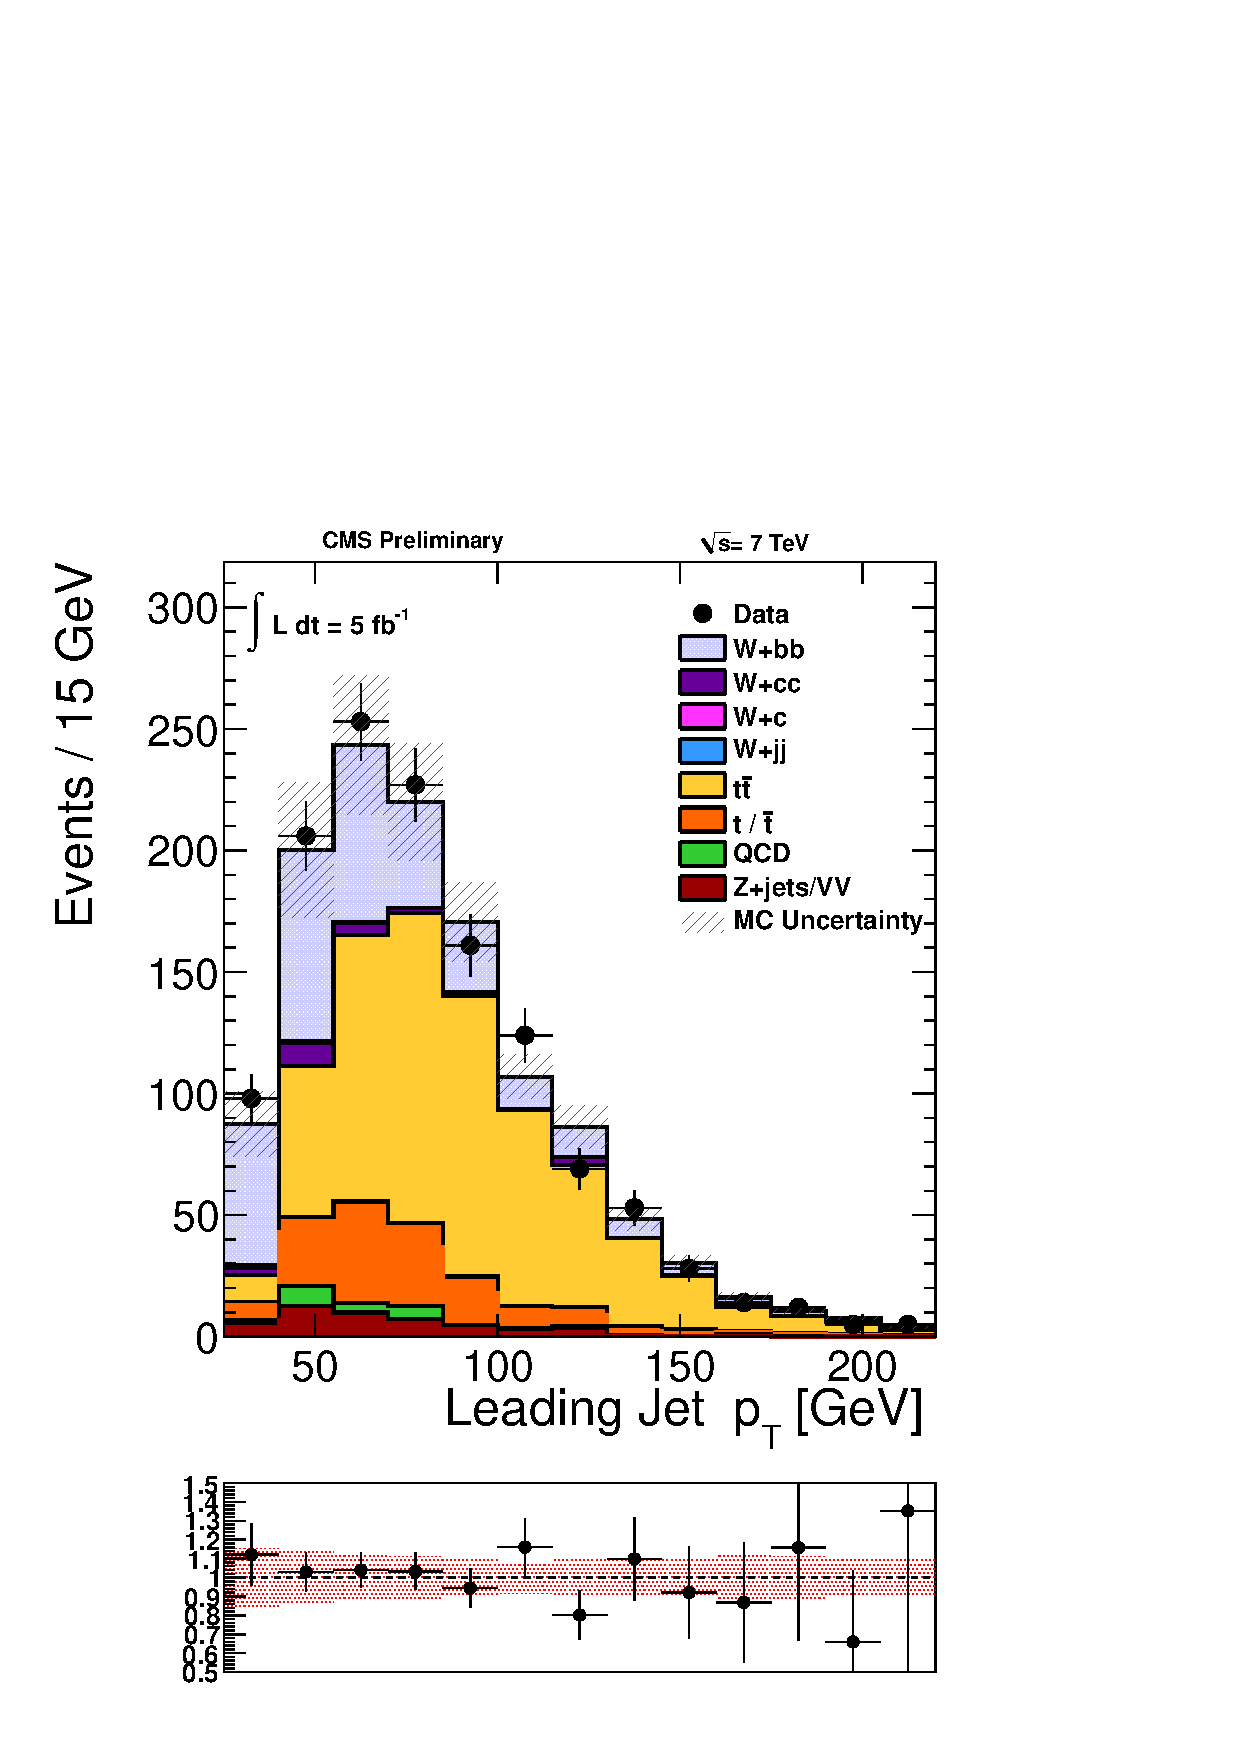
\includegraphics[width=0.45\textwidth, trim = 0 4cm 0 0, clip=true ]{Wbb/fig4.pdf}
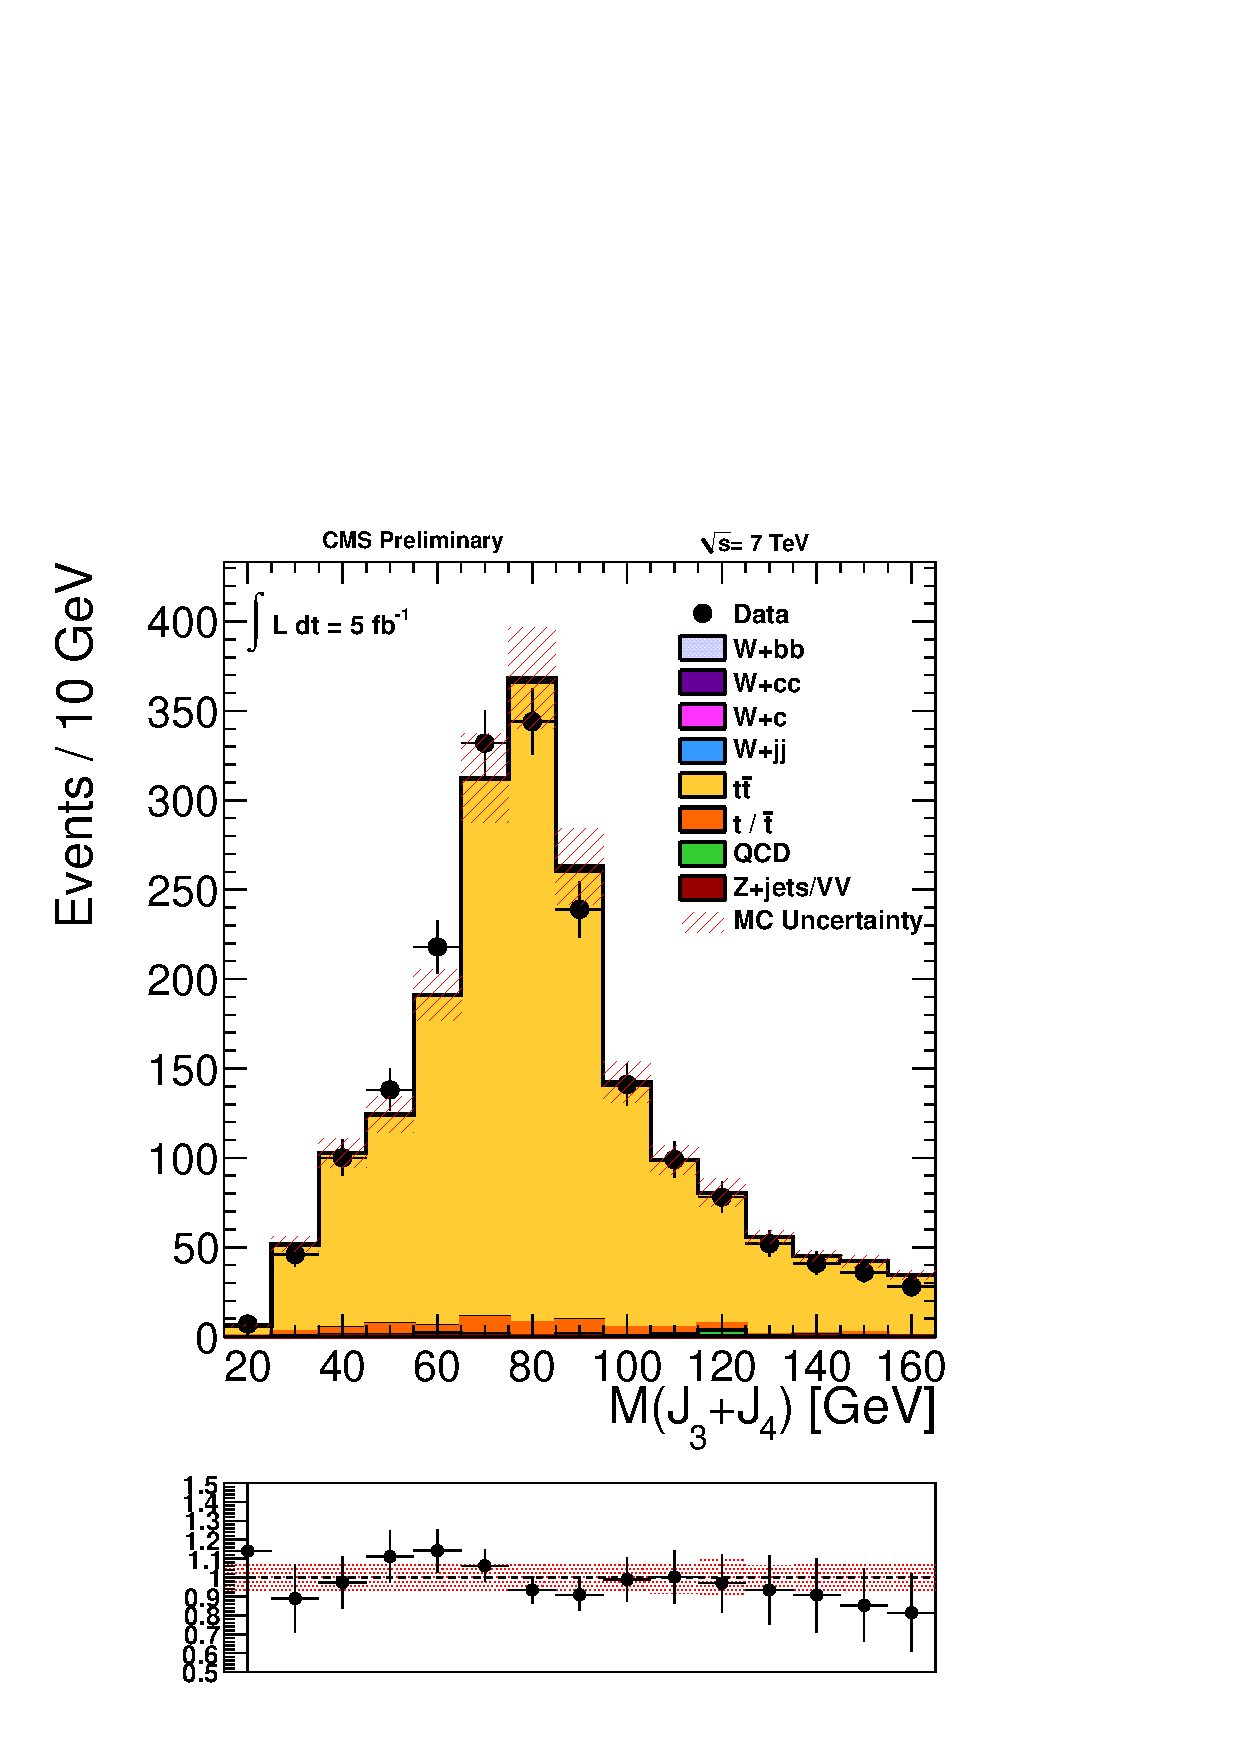
\includegraphics[width=0.45\textwidth, trim = 0 4cm 0 0, clip=true ]{Wbb/fig3.pdf}
\caption{ 
(left) The $\pt$ distribution of the highest-$\pt$ jet in the signal region, normalized to the result of the binned maximum likelihood fit.
(right) The invariant mass of the two additional light jets in the $\ttbar$ control region, also
normalized to the results of the fit.
}
\label{fig:figB}
\end{figure}

The final yields are extracted via a binned maximum likelihood fit.
To constrain the most prominent backgrounds and reduce the final
systematic uncertainty the fit is performed simultaneously on the $\pt$ of the leading jet ($\rm{J_1}$) 
in the signal region after all selection requirements have been applied,
and on the $m_{\rm{J_3 J_4}}$ distribution obtained from the $\ttbar$ control region.
The  $\rm{J_1}$ $\pt$  is chosen as the final fit variable due to its discrimination power against top-related backgrounds.
Figure~\ref{fig:figB} shows the two fitted distributions, $\pt^{\rm{J_1}}$  in the signal region (left)
and $m_{\rm{J_3 J_4}}$ in the $\ttbar$ control region (right), normalized to the results of the fit.

The statistical and systematic uncertainties are introduced in the form of
nuisance parameters via log-normal distributions around the estimated central values.
The fitted yields for each one of the processes can be found in Table~\ref{tab:fitYields}, 
compared to the Monte Carlo predictions.
To calculate the final uncertainties, first the          
total errors are calculated by taking both
the statistical and systematic errors into
account in the fit. Then the systematic nuisance parameters are removed, the fit is re-run
and the statistical uncertainty is 
obtained. The total systematic error is calculated by subtracting in quadrature 
the statistical uncertainty from the total error.
%I am not sure we need this, I think it is irrelevant...


%\begin{table}[htb]
%\begin{tabular}{|c|c|c|c|c|c|c|c|c|c|}
%\hline
%Process                &\Wbb         &W+light          & \Wcc           &Z+jets        &$t\bar{t}$    &Single Top     & VV             &QCD      & Total  \\
%\hline
%Prediction             & 332        & 1.5             & 21          & 31            &596          &160           &19           &33         & 1194   \\
%                       & $\pm66$    & $\pm 0.2$       &$\pm4$       &$\pm 3$        &$\pm35$      &$\pm 13$      &$\pm 3$      &$\pm 17$   & 78  \\
%\hline
%Fitted                 &300         &1                & 20          &32             &647          &170           &17           &33         & 1220  \\
%Yields                 &-56/+63     & $\pm1$          & $\pm 4$     & $\pm 3$       & $\pm 52$    & $\pm 13$     & $\pm 3$     & $\pm 16$  & -79/+84  \\
%\hline
%\end{tabular}
%\caption{Comparison of the expected (before the fit) and measured (after the fit) yields for each of the processes. The uncertainty on 
%the Monte Carlo prediction takes into account the variation allowed in the background contributions in the fit. The uncertainty in the fitted yields
%corresponds to the full uncertainty after the fit.
%}
%\label{tab:fitYieldsHorizontal}
%\end{table}

\begin{table}[htb]
\begin{center}
\begin{tabular}{c c c }
\hline 
Process  & Prediction  & Fitted Yield \\
\hline 
$\Wbb$         & $332\pm66$     & $300\pm60$ \\
$\Wc$, $\Wcc$  & $21\pm4$       & $20\pm4$ \\
W+usdg         & $1.5\pm0.2$    & $1\pm1$  \\
Z+jets         & $31\pm3$       & $32\pm3$ \\   
$\ttbar$       & $596\pm35$     & $647\pm52$ \\  
Single top     & $160\pm13$     & $170\pm13$ \\
WW, WZ         & $19\pm3$       & $17\pm3$   \\
QCD            & $33\pm17$      & $33\pm16$  \\
\hline
Total          & $1194\pm78$    & $1220\pm82$ \\ 
\hline 
\hline
Observed Events & \multicolumn{2}{c}{$1230\pm35 $} \\
\hline 
\end{tabular}
\caption{Comparison of the expected (before the fit) and measured (after the fit) yields for each of the processes. The uncertainty on
the Monte Carlo prediction takes into account the variation allowed to the nuisance parameters in the fit. The uncertainty in the fitted yields
corresponds to the full uncertainty after the fit.
}
\label{tab:fitYields}
\end{center}
\end{table}

The observed number of events in data after selection in the signal region is $N(S+B)_{data}=1230\pm35 $. 
The number of signal events obtained in the binned maximum likelihood fit is $300\pm60$. 

To show the robustness of the $\Wbb$ fit result a separate study was performed with
two selected b-tagged jets that require each jet to fulfill a looser CSV b-tagging criterion, corresponding 
to an efficiency  of 70\%
for jets containing b-flavored hadrons, while the misidentification probability for light-quark jets is 1$\%$.
%%%% Note that TOP-12-024 quotes 60% - 1% 
With the exception of the modification to the CSV threshold, all other selections for the signal
and control region remain unchanged. The $\Wcc$ contribution is non-negligible with this selection,
therefore, the sum of the invariant mass of the secondary vertex found in each selected jet
is used to distinguish between $\Wbb$ and $\Wcc$. The scalar sum of the transverse momenta of the
muon, the $\vecEtm$ and the jets,
$H_{\rm{T}}$, is used to distinguish W+jets from
top contributions. 
The $\Wbb$ signal is extracted via a two dimensional fit of 
$H_{\rm{T}}$ versus
the sum of the the  secondary vertex masses of the highest- ($\rm{J_1}$) and second-highest-$\pt$ ($\rm{J_2}$) jets. 
An equivalent $\ttbar$ control region to the one described in the
tighter selection, based on the reconstruction of the W mass using two light jets, is also used in this case.
The variables $\rm{J_1}$ SV mass + $\rm{J_2}$ SV mass and $H_{\rm{T}}$ are shown in Fig.~\ref{fig:figC}, with yields 
normalized to the results of the fit.
%The fit yield obtained for the $\Wbb$ signal with this alternate selection is 
%$1.13\pm  0.09\stat ^{+0.18}_{-0.17}\syst \pm 0.18 \theo \pm 0.03\lumi \unit{pb.}$.%$\sigma_{\Wbb}=0.867 \pm 0.07 (stat.) ^{-0.129}_{+0.140} (syst.)$. 
%Background processes predicted by
%Monte Carlo are found to change less than 0.3$\sigma$ with the exception of the $\Wcc$ background 
%whose yield is shifted up by 10\%. 
The cross section value computed with this alternative method 
is found to be consistent
with the primary fit results quoted above.

\begin{figure}
\centering
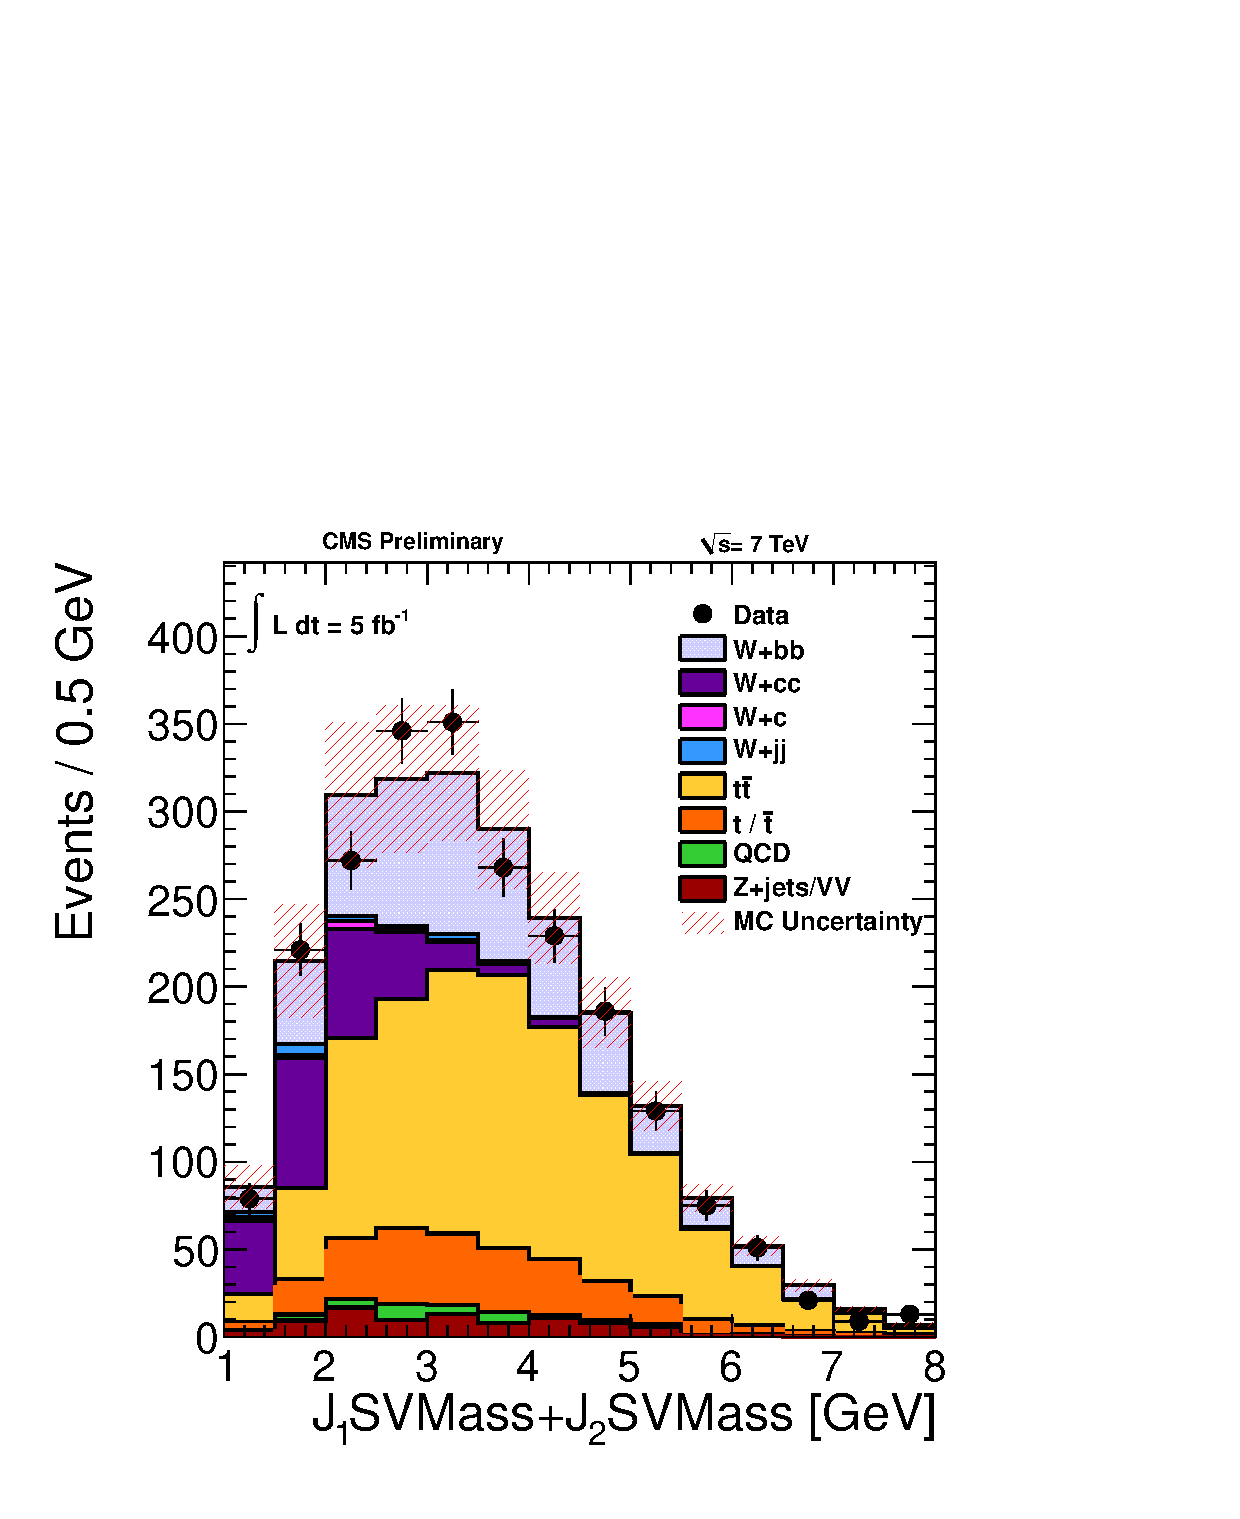
\includegraphics[width=0.45\textwidth]{Wbb/fig3a.pdf}
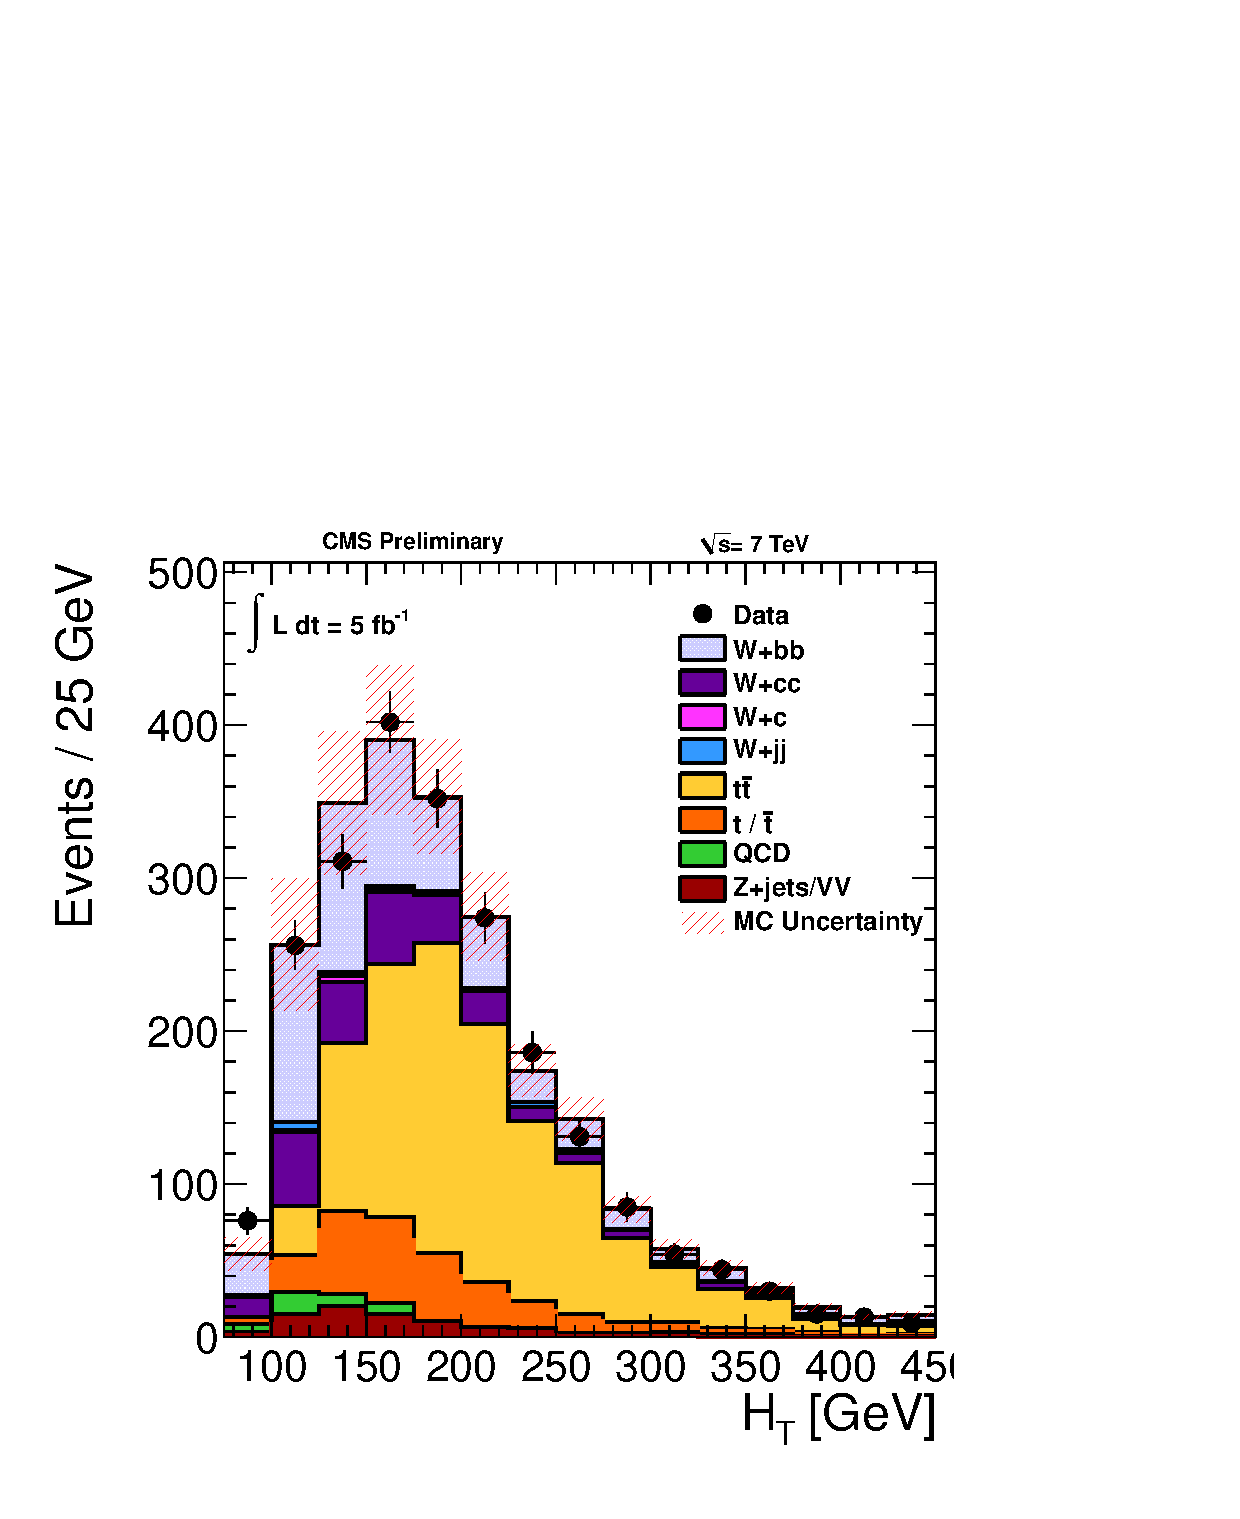
\includegraphics[width=0.45\textwidth]{Wbb/fig4a.pdf}
\caption{
The distribution of the sum of the masses of the two secondary vertices ($\rm{J_1}$ SV mass + $\rm{J_2}$ SV mass) (left)  and $H_{\rm{T}}$ of the system (right) in the alternative
medium b-tag selection, 
normalized to the results of the cross-check fit. 
%To further distinguish between $\Wbb$ and $\Wcc$ we introduce the variable '$J_{1}$ SV mass + $J_{2}$ SV mass',
%this is simply the sum of the invariant masses of the secondary vertex found in each selected jet. (left)
%The distribution of $J_{1}$+$J_{2}$ SV mass in the alternate two medium b-Tag selection is shown with yields after the fit;
%the $J_{1}$+$J_{2}$ SV mass variable provides powerful discrimination of $\Wbb$ and $\Wcc$ in this
%selection where there are looser b-tagging requirements. 
%(right) Distribution of $J_{1}$+$J_{2}$ SV mass in the two tight b-Tag selection.
}
\label{fig:figC}
\end{figure}

The $\Wbb$ cross section within the reference fiducial phase space
is determined using the following equation:
\begin{equation*} 
\sigma(pp\rightarrow \Wbb) = \frac{N_{Data}-N_{Bckg}}{\Lint~\epsilon_{sel}},
\nonumber
\end{equation*}
where the efficiency of the selection requirements $\epsilon_{sel} = 10.4 \pm 1.0\%$
is estimated with \MADGRAPH. The associated errors correspond to PDFs and to the factorization/matching scales.

The measured cross section is
%, unfolded to the b-hadron level as described above, for muons with
%$\pt > 25\GeV$ and $|\eta|<2.1$ and two b-jets with
%$\pt > 25\GeV$ and $|\eta|<2.4$ is found to be 
%$1.17\pm  0.11\stat ^{+0.21}_{-0.17}\syst \pm 0.18 \theo \pm 0.03\lumi \unit{pb.}$
\begin{eqnarray*}
\sigma(pp\rightarrow \mathrm{W} + \bbbar, p_T^{\mathrm{b}}>25~\GeV, |\eta^{\mathrm{b}}|<2.4)\times{\cal{B}}(\Wmn, p_T^{\mu}>25~\GeV, |\eta^\mu|<2.1) = \\
            =0.53\pm  0.05\stat \pm 0.09 \syst \pm 0.06 \theo \pm 0.01\lumi \mathrm{pb.} %(FIXME!!! where do we quote the errors of Q2?).
\end{eqnarray*}

%The \MADGRAPH  cross sectioni (FIXME!!! where do we quote the errors of Q2?),
%corrected to the NNLO using the standard reference
%cross-section value in CMS (FEWZ, MSTWNNLO), is
%estimated to be $1.30\pm0.09$ pb (no vetoes) or $0.58\pm0.08 $ pb  (vetoes). 
This cross section is calculated at the level of final-state particles, by requiring a muon with $p_T>25\GeV$ and $|\eta|<2.1$ and
exactly two jets, reconstructed using the anti-$k_T$ jet algorithm with distance parameter 0.5, with $p_T>25\GeV$ and $|\eta|<2.4$ and
each containing at least one b hadron with $p_T>5\GeV$. Events with extra jets are vetoed.
A hadronization correction factor $0.92\pm0.01$ to extrapolate from the final-state particle jets 
%b-hadron measurement 
to the parton-level cross section 
is estimated with \MADGRAPH+\PYTHIA. At the parton level the events are required to have a 
muon with
$\pt > 25\GeV$ and $|\eta|<2.1$ and exactly two parton-jets with
$\pt > 25\GeV$ and $|\eta|<2.4$ each containing a b parton just before hadronization. This factor has been computed in the 4-flavor and 5-flavor
schemes, and the difference between said calculations is assigned as systematic uncertainty to the measurement.
The simulated partons include double parton scattering and multiple parton interaction 
production of $\bbbar$ pairs, which have been found to reproduce adequately these 
processes observed by CMS measurements. 

The measured values can be compared to the NLO cross section of
%\begin{displaymath}
%$0.94 ^{+0.20}_{-0.15}pb.$
$0.52 \pm 0.03pb.$ 
%\end{displaymath}
calculated with MCFM~\cite{Campbell:2010ff, Badger:2010mg}.
The MCFM cross section is calculated using the MSTW2008NNLO~\cite{Martin:2009iq} PDF, and 
setting the normalization and renormalization scales to $\mu_{\rm{F}} = \mu_{\rm{R}} = m_{W} + 2m_{\rm{b}}$.
The theoretical cross section uncertainties
are estimated by varying the $\mu_{\rm{F,R}}$ simultaneously up and down by a factor of two, and also take
into account PDF uncertainties computed using standard procedures.

%Correction factors to go from this fiducial measurement to the full phase-space can be computed with MCFM.
%The acceptance correction to extrapolate the measurement in $p_T^{\mu}>25~\GeV$ and $|\eta^{\mu}|<2.1$ to
%the full muon phase-space is found to be ${\cal{A}}(\mu)=0.50\pm XX \textrm{PDF}$. The acceptance correction 
%to remove the veto on extra jets is found to be ${\cal{A}}(\textrm{jet~veto})=0.50\pm XX \textrm{$\mu_{\rm{F,R}}$}$.

\begin{figure}
\centering
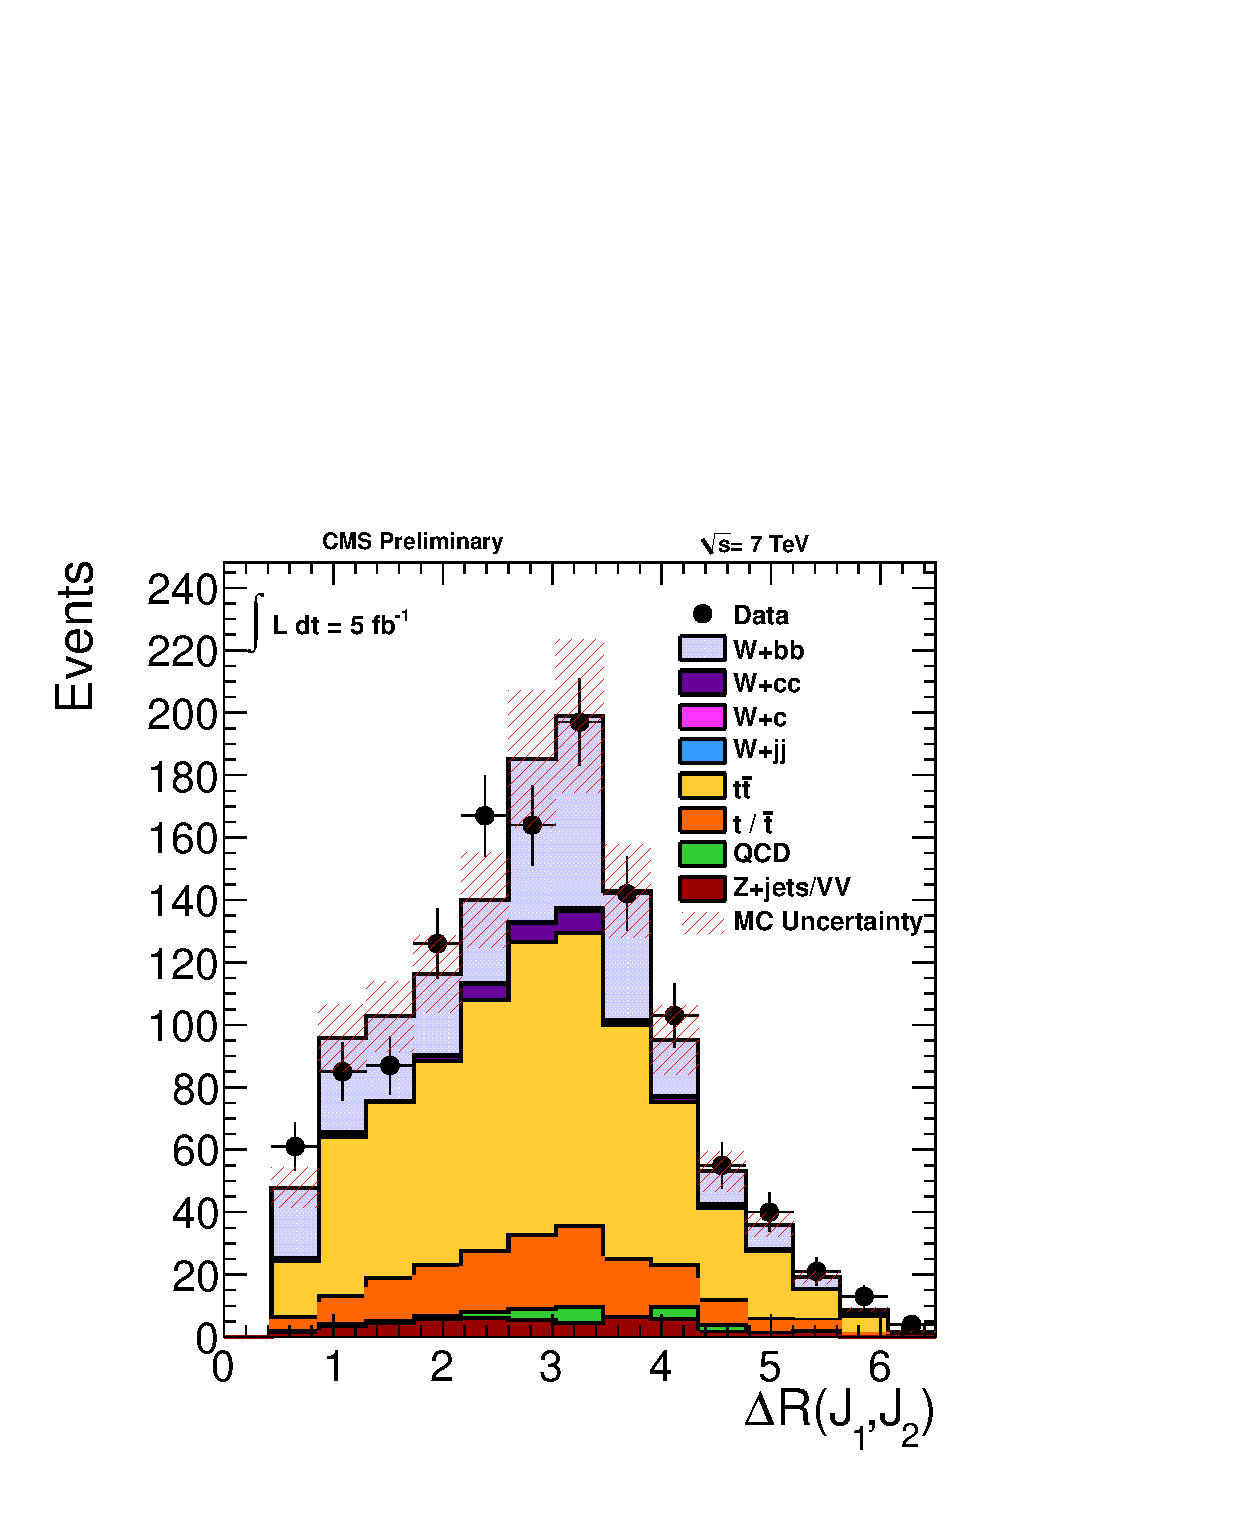
\includegraphics[width=0.45\textwidth]{Wbb/fig5.pdf}
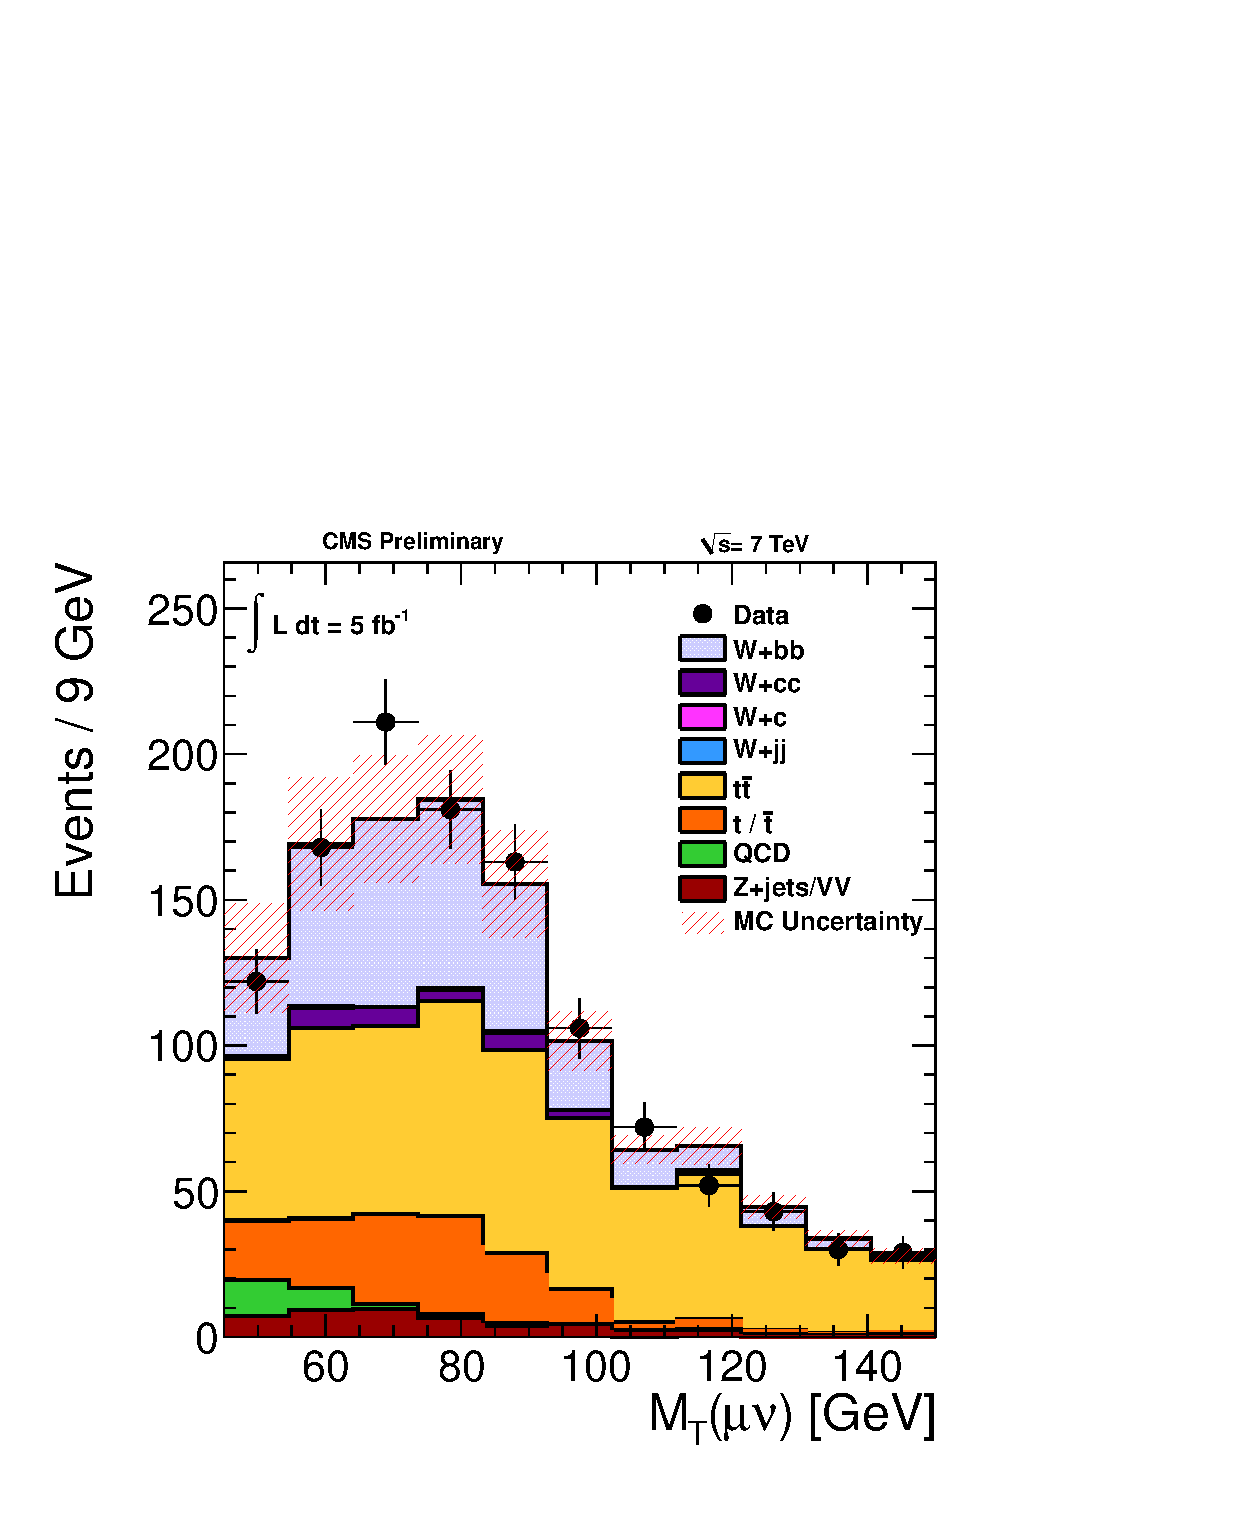
\includegraphics[width=0.45\textwidth]{Wbb/fig6.pdf}
\caption{(left) The $\Delta R$ between the two selected b jets
(right) the $\MT$ distribution, normalized to the results of the fit.}
\label{fig:figD}
\end{figure}

In addition to this measurement of the cross section, we have explored the kinematics of the $\Wbb$ system.
The angular distance between two selected b jets, $\Delta R(\rm{J_1,J_2})$ 
and the $\MT$ distribution are compared to Monte Carlo predictions 
in Fig.~\ref{fig:figD}. The shapes are taken from simulation and are normalized to the fit results. 
Figure~\ref{fig:figE} shows the invariant mass of the two 
selected b jets system and its $\pt$.
The observed distributions  are well described by the simulation.
%Those distributions are very important for the dominant background background estimation
%in the $WH\rightarrow l \nu b \bar{b}$ search.


%The measured cross section, unfolded to the b-hadron level as described above, for muons with
%$\pt > 25\GeV$ and $|\eta|<2.1$ and two b-jets with
%$\pt > 25\GeV$ and $|\eta|<2.4$ is found to be 
%$1.17\pm  0.10\stat ^{+0.21}_{-0.17}\syst \pm 0.09 \theo \pm 0.03\lumi \unit{pb.}$

% No quoting MCFM until we fix the C(parton, hadron) factor

In summary, we have presented a measurement of the $\Wbb$ production
cross section in proton-proton collisions at 7\TeV. The W+$\bbbar$ events
have been  selected in the W $\to \mu\nu$ decay mode with a 
muon of $\pt>25\GeV$ and $|\eta|<2.1$, and two b jets with $\pt>25\GeV$ and $|\eta|<2.4$. 
The data sample corresponds to an integrated luminosity of $5.0\fbinv$.
%The measured cross section
%$\sigma ( \Wbb) =  0.98 \pm 0.12 \stat \pm0.20 \syst \pm 0.07 \theo \pm 0.02\lumi pb.$
%is consistent with the SM prediction.
The measured cross section 
%$\sigma ( \Wbb) =  0.98 \pm 0.12 \stat \pm0.20 \syst \pm 0.07 \theo \pm 0.02\lumi \unit{pb}$
%$\sigma ( \Wbb) = 1.17\pm  0.10\stat ^{+0.21}_{-0.17}\syst \pm 0.18 \theo \pm 0.03\lumi \unit{pb.}$
$\sigma(pp\rightarrow \mathrm{W} + \bbbar, p_T^{\mathrm{b}}>25~\GeV, |\eta^{\mathrm{b}}|<2.4)\times {\cal{B}}(\Wmn, p_T^{\mu}>25~\GeV, |\eta^{\mu}|<2.1) =0.53\pm  0.05\stat \pm 0.09 \syst \pm 0.06 \theo \pm 0.01\lumi pb.$
for production of a W boson in association with two b jets is in agreement with
the SM predictions.
This result is approaching the precision of theoretical predictions at NNLO, 
allowing a sensitive test of perturbative calculations
in the SM.


\begin{figure}
\centering
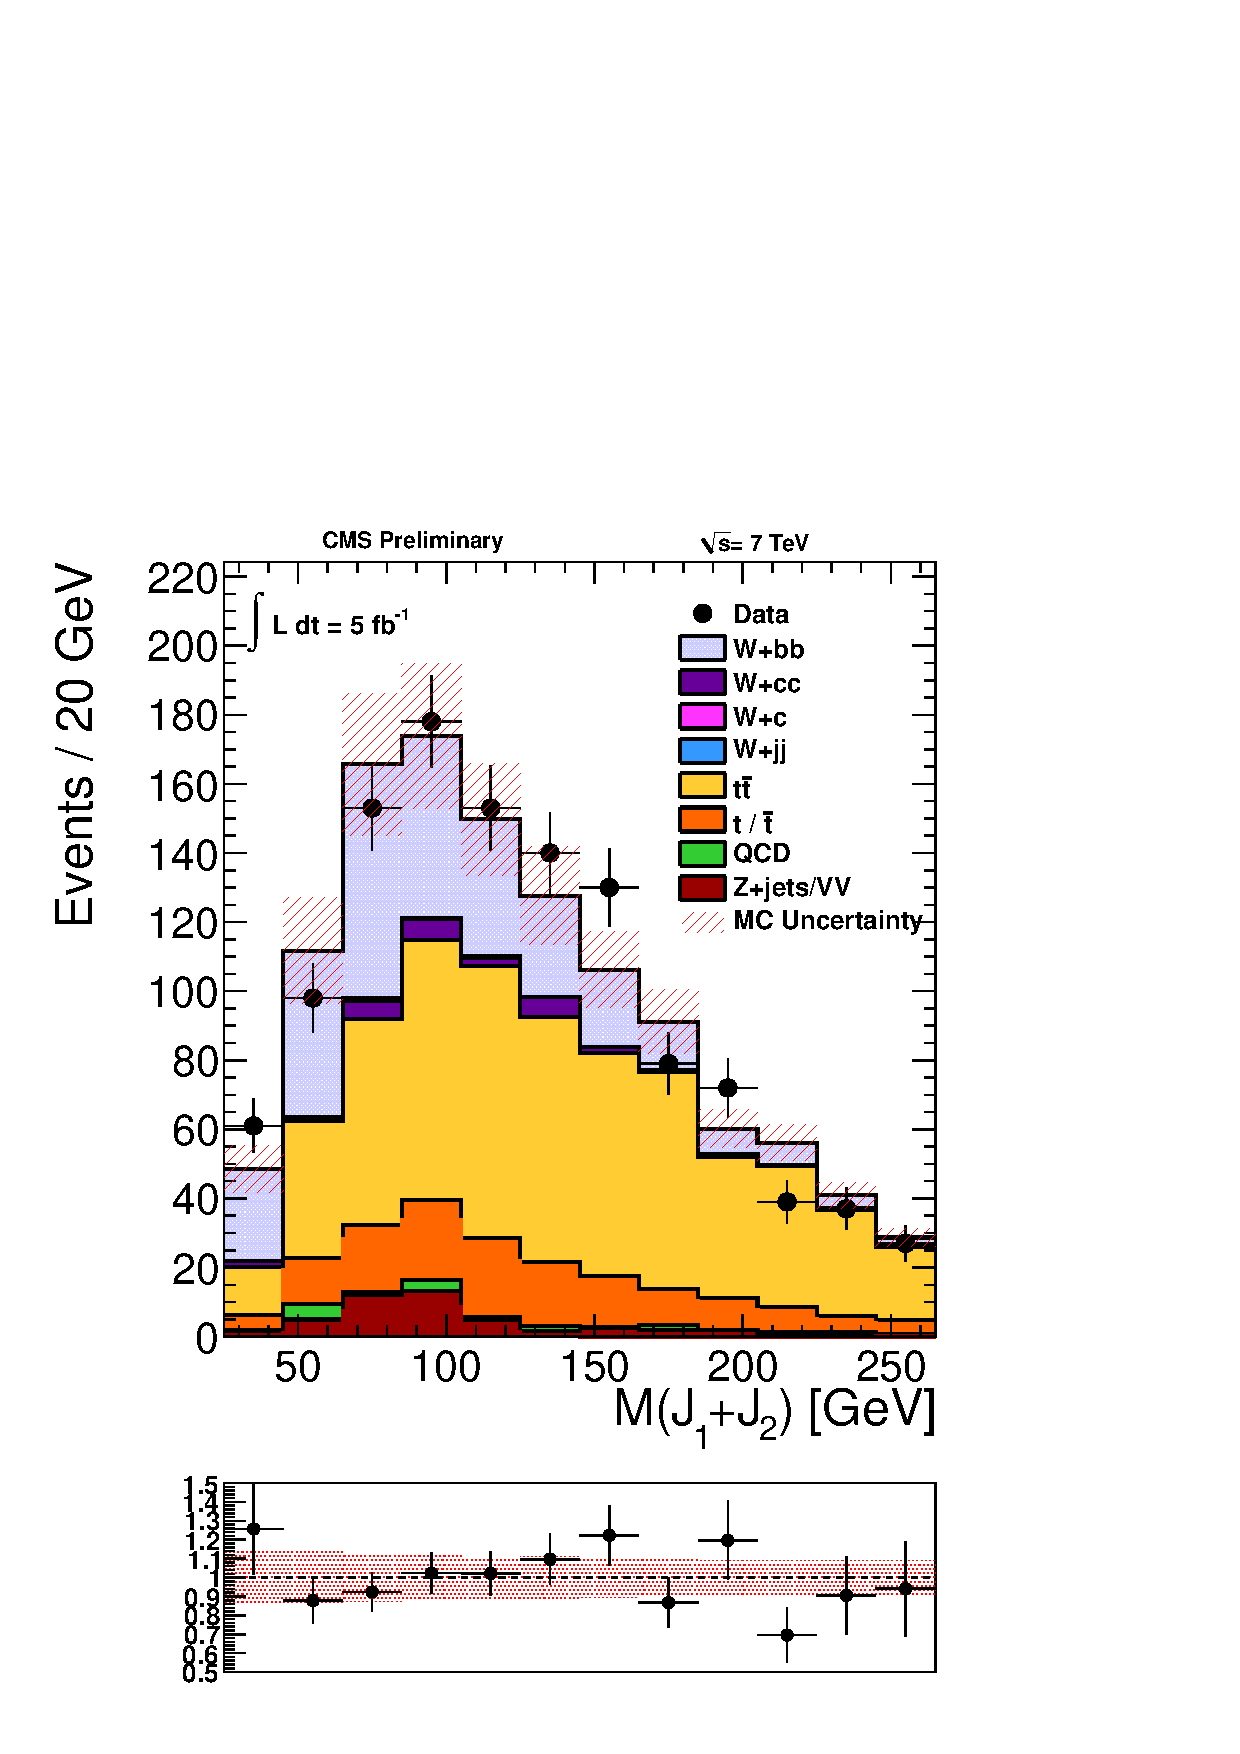
\includegraphics[width=0.45\textwidth, trim = 0 4cm 0 0, clip=true ]{Wbb/fig7.pdf}
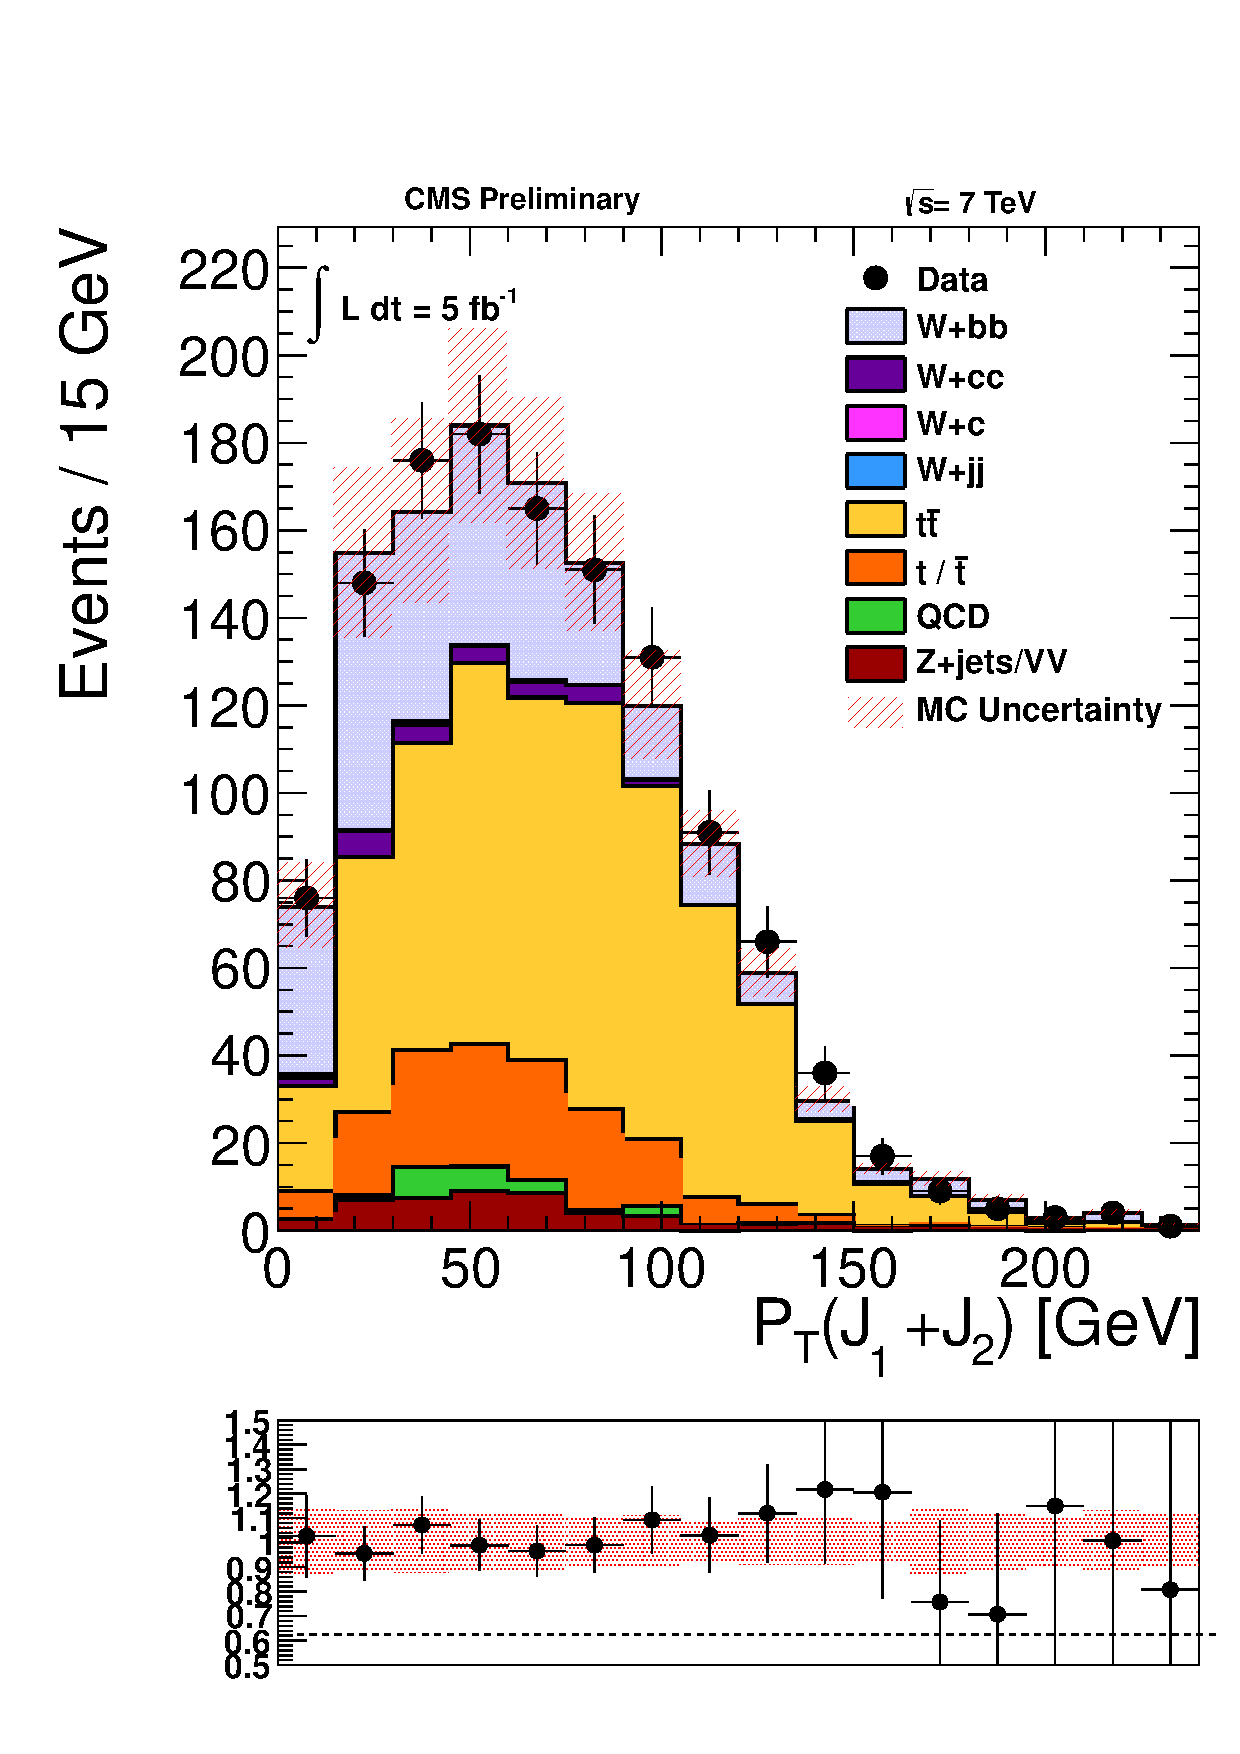
\includegraphics[width=0.45\textwidth, trim = 0 5cm 0 0, clip=true ]{Wbb/fig8.pdf}
\caption{(left) The invariant mass, $m_{\rm{J_{1} J_{2}}}$ of the two selected b jets and 
(right) the $p_{T}(J_{1} J_{2})$ distribution, normalized to the results of the fit.}
\label{fig:figE}
\end{figure}
